\documentclass[12pt,a4paper]{article}
\usepackage[utf8]{inputenc}
\usepackage[german]{babel}
\usepackage[T1]{fontenc}
\usepackage{amsmath}
\usepackage{amsfonts}
\usepackage{amssymb}
\usepackage{graphicx}
\usepackage{siunitx}
\usepackage{float}
\usepackage[left=2cm,right=2cm,top=2cm,bottom=2cm]{geometry}
\author{Gerald}

\begin{document}
\sisetup{separate-uncertainty = true}
	\setlength{\parindent}{0pt} 
	\begin{center}
		{\LARGE Versuchsprotokoll}\\
		\begin{large}
			zum Fortgeschrittenenpraktikum im Bachelorstudiengang Physik\\[0.4cm]
			an der RWTH Aachen\\
			II. Physikalisches Institut A\\[5.5cm]
			\Large\textbf{\textsl{Rastertunnelmikroskopie (STM)}}\\[5.5cm]
			\normalsize\textit{vorgelegt\\von}\\[0.4cm]
			\large{Moritz Berger (355244)\\Gerald Kolter (355005)}\\Gruppe 30\\[2cm]
			\large \textbf{Wintersemester 2017/18}
		\end{large}
	\end{center}
	\newpage
	
	\tableofcontents
	\newpage

\section{Versuchsziel}
Das Ziel des Versuchs besteht darin, mit einem Rastertunnelmikroskop bei der Vermessung einer Goldprobe die Auswirkung der Einstellungen auf das Messergebnis zu untersuchen. Mit einer Probe eines hochorientierten pyrolytischen Graphit (HOPG) wird der Abstand der Gitterebenen bestimmt und eine Kalibration in x- und y-Richtung durchgeführt.

\section{Aufbau}
Das verwendete Rastertunnelmikroskop besteht aus einem Halter für die Platin-Iridium-Spitze, der mit piezoelektrischen Kristallen in allen drei Raumrichtungen bewegt werden kann, und einem Probenhalter, der auf einem sogenannten Schrittmotorantrieb liegt. Dieser funktioniert ebenfalls mit einem piezoelektrischen Kristall und dient lediglich der Grobannäherung. Spitze und Probe sind über eine Spannungsquelle verbunden, wobei gleichzeitig der in diesem Kreis fließende Strom gemessen wird. Dieser Strom kommt bei kleinen Abständen zwischen Spitze und Probe durch den Tunneleffekt zustande. Die Abhängigkeit zwischen Strom und Abstand ist exponentiell und damit sehr stark.\\
Die Spitze wird mit den piezoelektrischen Kristallen über die Probe gerastert, wobei jede Linie in x-Richtung vorwärts und rückwärts abgefahren wird.\\
Eine Regelungselektronik steuert die z-Richtung der Spitze in Abhängigkeit des Tunnelstroms. Dabei gibt der sogenannte I-Gain an, wie schnell die Regelung auf kurze Pulse reagiert.

\section{Durchführung}
\subsection{Untersuchung der Mikroskopeigenschaften mit einer Goldprobe}

\begin{table}
\centering
\begin{tabular}{|c|c|}
\hline 
Bereichgröße & (75,23 nm)$^2$ \\ 
\hline 
Zeit pro Linie & 0,2 s \\
\hline 
Tunnelspannung & 450 mV \\ 
\hline 
Messpunkte pro Linie & 256 \\
\hline 
Sollwert Tunnelstrom & 1 nA \\
\hline 
\end{tabular} 
\caption{Einstellungen der Messparameter bei Vermessung der Goldprobe. Bei dieser Messreihe wurde der I-Gain zwischen 1000 und 11000 verändert.}
\label{tab:IGain_Einstellungen}
\end{table}

Für die Untersuchung der Empfindlichkeit der Einstellparameter wird auf der Goldprobe zunächst ein Bereich mit markanter Struktur gesucht. Dieser Bereich wird für vier verschiedene Werte für den I-Gain bei ansonsten gleichbleibenden Parametern vermessen. Diese Einstellungen sind in Tabelle \ref{tab:IGain_Einstellungen} eingetragen. Es wurden vier verschiedene Einstellungen für den I-Gain verwendet: $I_1 = 1000$, $I_2 = 3000$, $I_3 = 8000$ und $I_4 = 11000$.\\
In einer zweiten Messreihe wird erneut ein Bereich mit markanter Struktur vermessen, wobei anstelle des I-Gain die Messzeit pro Zeile verändert wird. Für den I-Gain wurde hierbei der Wert, der sich in der ersten Messreihe als beste Annäherung des Idealwertes herausgestellt hat, verwendet (I-Gain = 3000). Alle anderen Parameter blieben unverändert. Es wurden sieben verschiedene Einstellungen für die Messzeit pro Zeile verwendet: $T_1 = \SI{52}{ms}$, $T_2 = \SI{80}{ms}$, $T_3 = \SI{100}{ms}$, $T_4 = \SI{200}{ms}$, $T_5 = \SI{400}{ms}$, $T_6 = \SI{600}{ms}$, $T_7 = \SI{2}{s}$.

\subsection{Untersuchung von HOPG}
\subsubsection{Vermessung einer Kante}
Auf der HOPG-Probe wird eine Kante in mehreren Auflösungen aufgenommen.

\subsubsection{Korrektur der Achsen über Atomabstände}
Die Achsenkalibration findet anhand der atomaren Abstände des Graphit-Gitters statt.\\
Um die Atome sehen zu können, muss eine Rastergröße im nm-Bereich gewählt werden.\\
Es wurden insgesamt 3 Aufnahmen mit unterschiedlichen Bereichsgrößen im Konstanthöhenmodus und 3 im Konstantstrommodus aufgenommen. Die dazugehörigen Messeinstellungen sind Tabelle \ref{tab:Atome_Einstellungen} zu entnehmen. Alle anderen Einstellungen wurden aus den anderen Versuchsteilen beibehalten.\\


\begin{table}
\centering
\begin{tabular}{|c|c|c|c|c|}
\hline 
Modus & Bereichsgröße[nm] & Zeilenzeit[s] & IGain & Tunnelspannung[mV]\\ 
\hline 
Höhen & 1 & 0.3 & 100 & 50.4\\ 
\hline 
Höhen & 2.325 & 0.3 & 100 & 50.4\\ 
\hline 
Höhen & 5 & 0.3 & 100 & 50.4\\ 
\hline 
Strom & 0.872 & 0.2 & 8000 & 50.4\\ 
\hline 
Strom & 2.325 & 0.2 & 8000 & 50.4\\ 
\hline 
Strom & 5 & 0.2 & 8000 & 50.4\\ 
\hline 
\end{tabular} 
\caption{Messeinstellungen aller Aufnahmen zu den Atomabständen.}
\label{tab:Atome_Einstellungen}
\end{table}

\section{Ergebnisse}
\subsection{Untersuchung der Mikroskopeigenschaften mit einer Goldprobe}

\begin{figure}
\centering
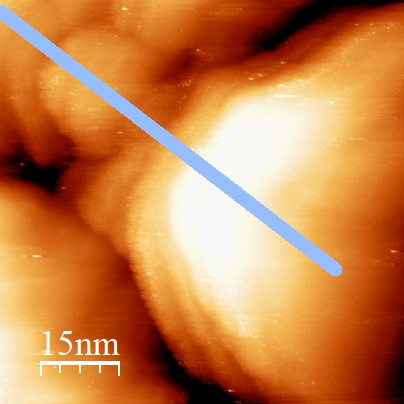
\includegraphics[scale=0.8]{Bilder/Anhang/IGain/3000_IGain_vor.jpg}
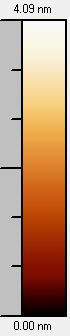
\includegraphics[scale=0.8]{Bilder/Anhang/IGain/3000_IGain_vor_Skala.jpg}
\caption{Bild der z-Komponente bei Vermessung der Goldprobe mit einem I-Gain von 3000 in der Vorwärtsrichtung. Der Balken quer im Bild verbildlicht die Stelle, aus der das Höhenprofil entnommen wurde.}
\label{fig:Gold_IGain_Beispiel}
\end{figure}

\begin{figure}
\centering
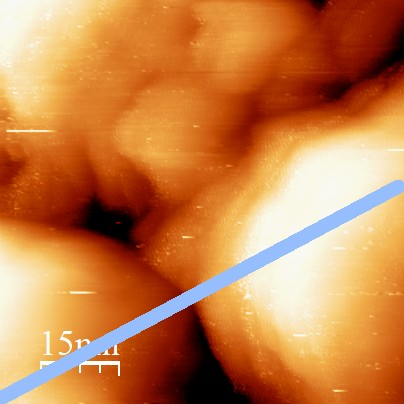
\includegraphics[scale=0.8]{Bilder/Anhang/Zeit/0_1_Zeit_vor.jpg}
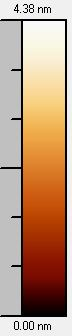
\includegraphics[scale=0.8]{Bilder/Anhang/Zeit/0_1_Zeit_vor_Skala.jpg}
\caption{Bild der z-Komponente bei Vermessung der Goldprobe bei einer Messzeit von 0,1s pro Linie in der Vorwärtsrichtung. Der Balken quer im Bild verbildlicht die Stelle, aus der das Höhenprofil entnommen wurde.}
\label{fig:Gold_Zeit_Beispiel}
\end{figure}

Abbildung \ref{fig:Gold_IGain_Beispiel} zeigt beispielhaft das Bild der z-Komponente nach Bearbeitung für eine Messung aus der Messreihe mit verändertem I-Gain. Der Balken quer im Bild zeigt, wo das im Folgenden untersuchte Höhenprofil entnommen wurde. In den Bildern aus den Ergebnissen der Messreihe wurde das Höhenprofil exakt gleich entnommen (Profillinie kopiert), sodass die Vergleichbarkeit der Profile gegeben ist.\\
Bei der Aufnahme der Messreihe mit veränderter Zeit wurde ein anderer Bereich verwendet. Daher ist die Profillinie aus einem anderen Bildbereich entnommen, wie in Abbildung \ref{fig:Gold_Zeit_Beispiel} dargestellt ist.\\
Bei der Entnahme des Höhenprofils wird für jeden Wert der Mittelwert mehrerer Punkte bestimmt.

\subsubsection{Bestimmung der Flankensteigung}
Zur Bestimmung der Flankensteigung werden die Punkte, die diese Flanke begrenzen, abgelesen.
Die Flankensteigung berechnet sich dann zu:

\begin{equation*}
a = \dfrac{Z_2 - Z_1}{X_2 - X_1}
\end{equation*}

Als Fehler auf die Werte wird der Ablesefehler

\begin{equation*}
\sigma = \dfrac{\SI{0.1}{nm}}{\sqrt{12}}
\end{equation*}

auf jeden abgelesenen Wert angenommen, sodass sich der Fehler auf die Steigung fortpflanzt zu:

\begin{equation*}
\sigma _a = \sqrt{2 \cdot \left( \dfrac{\sigma}{X_2 - X_1} \right) ^2 + 2 \cdot \left( \sigma \cdot  \dfrac{Z_2 - Z_1}{(X_2 - X_1)^2} \right) ^2}
\end{equation*}


\subsubsection{Untersuchung der Auswirkungen des I-Gain}

\begin{table}
\centering
\begin{tabular}{|c|c|c|}
\hline 
IGain & Peakpositionen in Vorwärtsrichtung [nm] & Peakpositionen in Rückwärtsrichtung [nm] \\ 
\hline 
1000 & (23.4, 0.0), (50.1, 3.4) & (27.5, 0.0), (44.7, 2.9) \\
\hline 
3000 & (36.5, 0.0), (48.2, 2.4) & (32.7, 0.0), (44.7, 2.6) \\ 
\hline 
8000 & (31.5, 0.0), (45.9, 4.4) & (28.0, 0.1), (44.0, 3.5) \\
\hline 
11000 & (30.8, 0.0), (48.6, 8.3) & (30.8, 0.0), (41.4, 9.4) \\
\hline 
\end{tabular} 
\caption{Abgelesene Werte für die Begrenzungen der Flanken in der Messreihe zur Variation des I-Gain.}
\label{tab:Peaks_IGain}
\end{table}

\begin{figure}
\centering
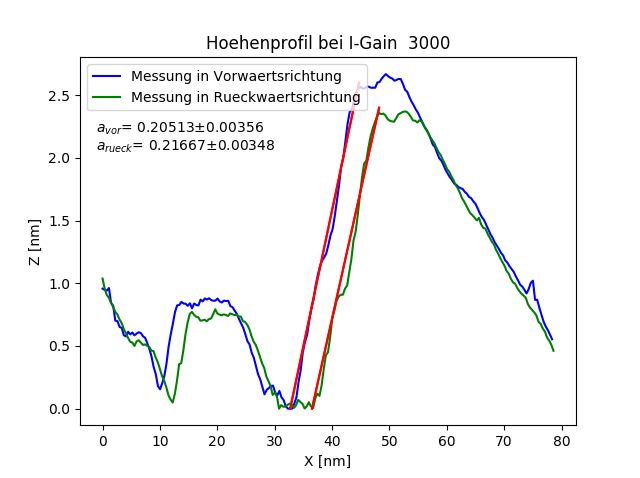
\includegraphics[scale=0.8]{Bilder/Anhang/IGain/Profil_IGain_3000.png}
\caption{Höhenprofil bei einem I-Gain von 3000. Die roten Linien markieren die abgelesenen Flanken.}
\label{fig:Gold_IGain_Flankensteigung}
\end{figure}

Tabelle \ref{tab:Peaks_IGain} zeigt alle abgelesenen Werte für diese Punkte in der Messreihe zum I-Gain. Abbildung \ref{fig:Gold_IGain_Flankensteigung} zeigt beispielhaft die gemessenen Höhenprofile und die abgelesenen Flanken bei einem IGain von 3000. 

\begin{table}
\centering
\begin{tabular}{|c|c|c|c|}
\hline 
IGain & $a_{vor}$ & $a_{rueck}$ & $\dfrac{|a_{vor} - a_{rueck}|}{\sqrt{\sigma _{a_{vor}}^2 + \sigma _{a_{rueck}}^2}}$ \\ 
\hline 
1000 & 0,1273 $\pm$ 0,0015 & 0,1686 $\pm$ 0,0024 & 14,44 \\
\hline 
3000 & 0,2051 $\pm$ 0,0036 & 0,2167 $\pm$ 0,0035 & 2,32 \\ 
\hline 
8000 & 0,3056 $\pm$ 0,0030 & 0,2125 $\pm$ 0,0026 & 23,57 \\
\hline 
11000 & 0,4663 $\pm$ 0,0025 & 0,8868 $\pm$ 0,0051 & 73,31 \\
\hline 
\end{tabular} 
\caption{Berechnete Flankensteigungen und die Abweichung zwischen der Steigung aus der Messung in Vorwärts- und der in Rückwärtsrichtung für die Messreihe mit variiertem I-Gain.}
\label{tab:Steigungen_IGain}
\end{table}

Tabelle \ref{tab:Steigungen_IGain} zeigt die Ergebnisse für die Flankensteigungen. Die Abweichungen zwischen den Steigungen aus der Messung in Vorwärts- und der in Rückwärtsrichtung zeigen, dass bei einer Messzeit von \SI{200}{ms} ein I-Gain von 3000 die besten Ergebnisse liefert.

\subsubsection{Untersuchung der Auswirkungen der Zeit}

\begin{table}
\centering
\begin{tabular}{|c|c|c|}
\hline 
Zeit [ms] & Peakpositionen in Vorwärtsrichtung [nm] & Peakpositionen in Rückwärtsrichtung [nm] \\ 
\hline 
52 & (33.0, 0.0), (51.1, 3.5) & (28.5, 0.0), (45.3, 3.4) \\
\hline 
80 & (22.2, 0.0), (54.8, 3.6) & (20.2, 0.0), (46.0, 3.5) \\ 
\hline 
100 & (38.6, 0.0), (54.2, 3.4) & (35.2, 0.0), (50.9, 3.7) \\
\hline 
200 & (18.7, 0.0), (53.8, 4.2) & (15.5, 0.0), (48.4, 4.2) \\
\hline 
400 & (36.5, 0.0), (53.1, 3.1) & (33.6, 0.0), (50.7, 3.5) \\
\hline 
600 & (27.6, 0.0), (52.7, 3.4) & (24.6, 0.0), (48.6, 3.3) \\
\hline 
2000 & (43.6, 0.0), (62.8, 3.1) & (38.8, 0.0), (57.0, 2.7) \\
\hline 
\end{tabular} 
\caption{Abgelesene Werte für die Begrenzungen der Flanken in der Messreihe zur Variation der Zeit.}
\label{tab:Peaks_Zeit}
\end{table}

\begin{figure}
\centering
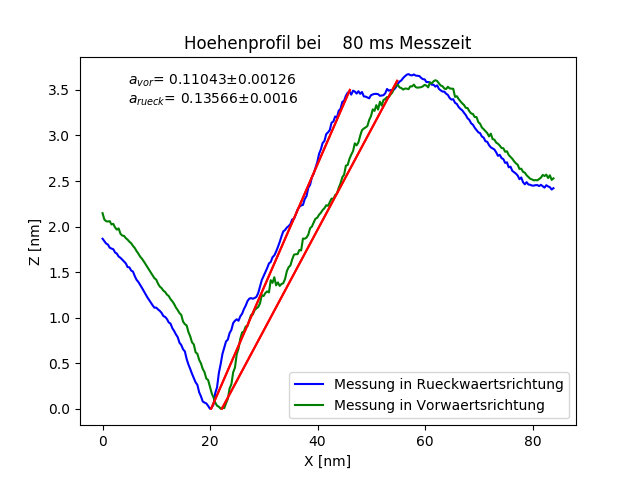
\includegraphics[scale=0.8]{Bilder/Profil_Zeit_80_Peakbestimmung.png}
\caption{Höhenprofil bei einer Messzeit von \SI{80}{ms}. Die roten Linien markieren die abgelesenen Flanken.}
\label{fig:Gold_Zeit_Flankensteigung}
\end{figure}

Tabelle \ref{tab:Peaks_Zeit} zeigt alle abgelesenen Werte für diese Punkte in der Messreihe zum I-Gain. Abbildung \ref{fig:Gold_Zeit_Flankensteigung} zeigt beispielhaft die gemessenen Höhenprofile und die abgelesenen Flanken bei einer Messzeit von \SI{80}{ms}.

\begin{table}
\centering
\begin{tabular}{|c|c|c|c|}
\hline 
Zeit [ms] & $a_{vor}$ & $a_{rueck}$ & $\dfrac{|a_{vor} - a_{rueck}|}{\sqrt{\sigma _{a_{vor}}^2 + \sigma _{a_{rueck}}^2}}$ \\ 
\hline 
52 & 0,1934 $\pm$ 0,0023 & 0,2024 $\pm$ 0,0025 & 2,67 \\
\hline 
80 & 0,1104 $\pm$ 0,0013 & 0,1357 $\pm$ 0,0016 & 12,40 \\ 
\hline 
100 & 0,2179 $\pm$ 0,0027 & 0,2357 $\pm$ 0,0027 & 4,68 \\
\hline 
200 & 0,1197 $\pm$ 0,0012 & 0,1277 $\pm$ 0,0013 & 4,67 \\
\hline 
400 & 0,1867 $\pm$ 0,0025 & 0,2047 $\pm$ 0,0024 & 5,13 \\
\hline 
600 & 0,1355 $\pm$ 0,0016 & 0,1375 $\pm$ 0,0017 & 0,86 \\
\hline 
2000 & 0,1615 $\pm$ 0,0022 & 0,1484 $\pm$ 0,0023 & 4,19 \\
\hline 
\end{tabular} 
\caption{Berechnete Flankensteigungen und die Abweichung zwischen der Steigung aus der Messung in Vorwärts- und der in Rückwärtsrichtung für die Messreihe mit variierter Zeit pro Zeile.}
\label{tab:Steigungen_Zeit}
\end{table}

Tabelle \ref{tab:Steigungen_Zeit} zeigt die Ergebnisse für die Flankensteigungen. Die Abweichungen zwischen den Steigungen aus der Messung in Vorwärts- und der in Rückwärtsrichtung zeigen, dass bei einem I-Gain von 3000 eine Messzeit pro Zeile von \SI{600}{ms} die besten Ergebnisse liefert.

\subsubsection{Stromprofil}

\begin{table}
\centering
\begin{tabular}{|c|c|c|c|c|}
\hline 
I-Gain & $\mu_{vor}$ [pA] & $\mu_{rueck}$ [pA] & $\sigma_{vor}$ [pA] & $\sigma_{rueck}$ [pA] \\ 
\hline 
1000 & 374,9 & 488,6 & 207,8 & 209,4 \\
\hline 
3000 & 220,1 & 249,3 & 99,1 & 84,9 \\ 
\hline 
8000 & 831,4 & 764,3 & 510,2 & 470,1 \\
\hline 
11000 & 728,3 & 676,2 & 641,2 & 610,5 \\
\hline 
\end{tabular} 
\caption{Mittelwert und Standardabweichung der Stromprofile in der Messreihe mit variiertem I-Gain.}
\label{tab:Strom_IGain}
\end{table}

\begin{table}
\centering
\begin{tabular}{|c|c|c|c|c|}
\hline 
Zeit [ms] & $\mu_{vor}$ [pA] & $\mu_{rueck}$ [pA] & $\sigma_{vor}$ [pA] & $\sigma_{rueck}$ [pA] \\ 
\hline 
52 & 877,7 & 752,2 & 329,0 & 276,2 \\
\hline 
80 & 329,1 & 322,6 & 123,8 & 111,0 \\ 
\hline 
100 & 388,4 & 668,3 & 177,6 & 190,8 \\
\hline 
200 & 275,9 & 342,3 & 117,8 & 99,8 \\
\hline 
400 & 179,2 & 168,4 & 55,2 & 53,6 \\
\hline 
600 & 179,9 & 173,5 & 60,7 & 55,5 \\
\hline 
2000 & 98,2 & 87,9 & 29,3 & 30,2 \\
\hline 
\end{tabular} 
\caption{Mittelwert und Standardabweichung der Stromprofile in der Messreihe mit variierter Messzeit pro Zeile.}
\label{tab:Strom_Zeit}
\end{table}

An der gleichen Stelle, an der aus dem Bild der z-Komponente das Höhenprofil entnommen wurde, kann aus dem Strombild ein Stromprofil entnommen werden. Anhand dieses Stromprofils kann durch Berechnen der Standardabweichung ebenfalls eine Aussage über die Güte des Bildes gemacht werden. Die Werte sind in den Tabellen \ref{tab:Strom_IGain} und \ref{tab:Strom_Zeit} dargestellt. \\
In der Messreihe mit dem variiertem I-Gain lässt sich leicht erkennen, dass die Standardabweichung bei einem I-Gain von 3000 einen minimalen Wert annimmt, daher kann hiermit das Ergebnis aus dem Vergleich der Flankensteigung bestätigt werden.\\
In der Messreihe mit der variierten Zeit sinkt die Standardabweichung mit der Messzeit pro Zeile. Dies liegt daran, dass bei konstantem I-Gain und steigender Messzeit pro Zeile der räumliche Bereich, der für die Regelung relevant ist, kleiner wird. Dadurch reagiert die Regelung örtlich gesehen schneller auf Veränderungen der Oberfläche, sodass der Probe-Spitze-Abstand weniger schwingt, was durch den hohen I-Gain und die große Zeit unterstützt wird.

\subsubsection{Zusammenfassung}
Mit steigendem I-Gain werden die gemessenen Flankensteigungen größer. Dabei liegt der ideale I-Gain in einem mittleren Bereich, wo die gemessenen Flankensteigungen aus der Vorwärts- und der Rückwärtsrichtung nahe zusammenrücken. \\
Bei der zweiten Messreihe mit Variation der Messzeit pro Zeile hat sich herausgestellt, dass bei einem I-Gain von 3000 und einer Messzeit von \SI{600}{ms} die Flankensteigungen aus der Vorwärts- und der Rückwärtsrichtung innerhalb einer Standardabweichung übereinstimmen.

\subsection{Untersuchung von HOPG}
Bei den Untersuchungen zum HOPG im Konstantstrommodus wurde ein IGain von 8000 verwendet, obwohl im Versuch mit Gold ein IGain von 3000 als optimal gefunden wurde. Dies liegt einerseits daran, dass hier feinere Strukturen aufgelöst werden müssen. Allerdings hat ein weiterer Effekt die Bilder mit einem niedrigerem IGain schlechter gemacht:\\
Beim IGain von 4000 ist die Anzahl an Fehllinien, die sich vom Untergrund abheben, wesentlich größer als bei einem IGain von 8000. Außerdem wird das Bild wesentlich unschärfer. Diese Effekte werden immer stärker, je kleiner der Rasterbereich gewählt wird.\\
Da beim annähern an das HOPG die Spitze gecrashed ist, vermuten wir, dass dieser Effekt durch eine schlechte Spitze entstehen kann. Die genaue Ursache ist aber unklar.\\
\\


\begin{figure}
\centering
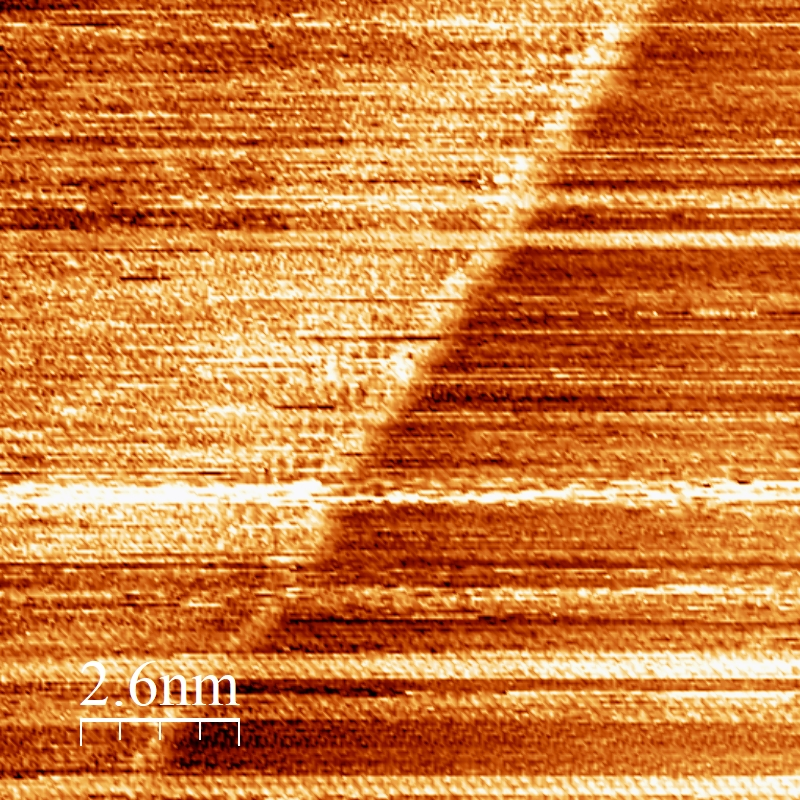
\includegraphics[scale=0.36]{Bilder/Igain4000.jpg}
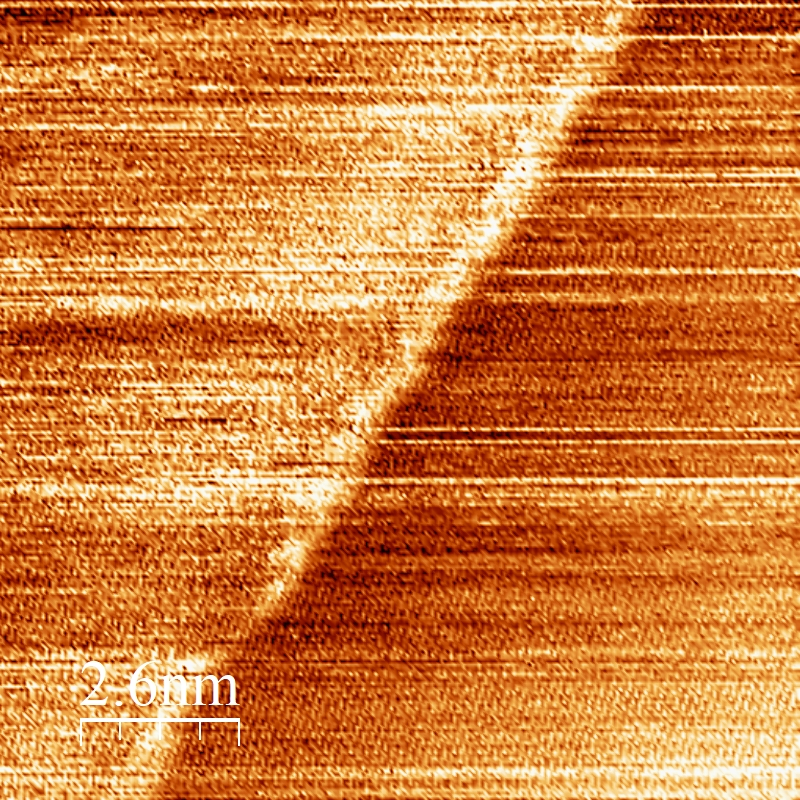
\includegraphics[scale=0.36]{Bilder/Igain8000.jpg}
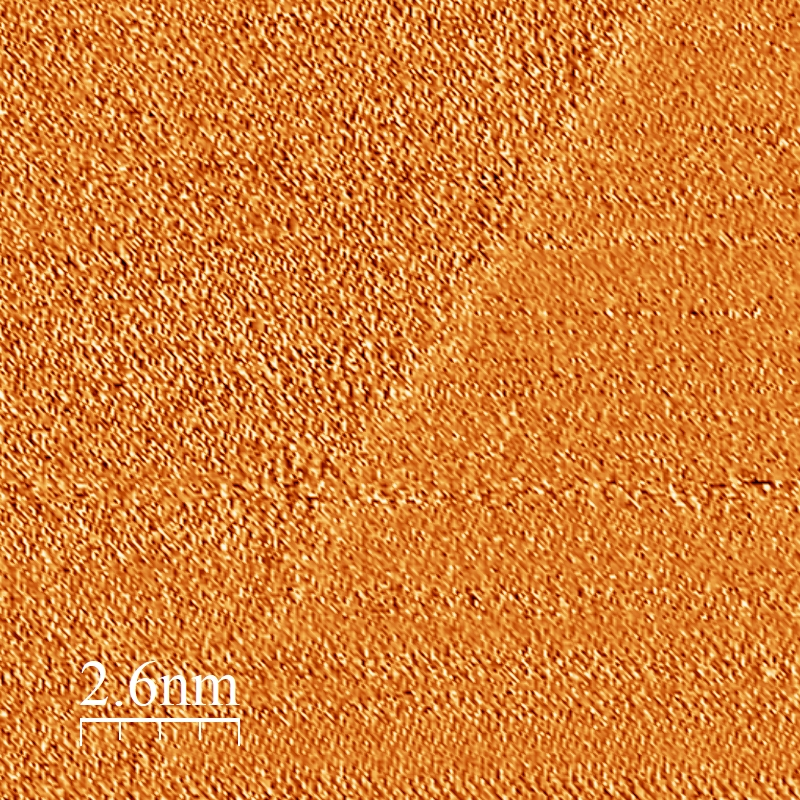
\includegraphics[scale=0.36]{Bilder/Igain4000_Strom.jpg}
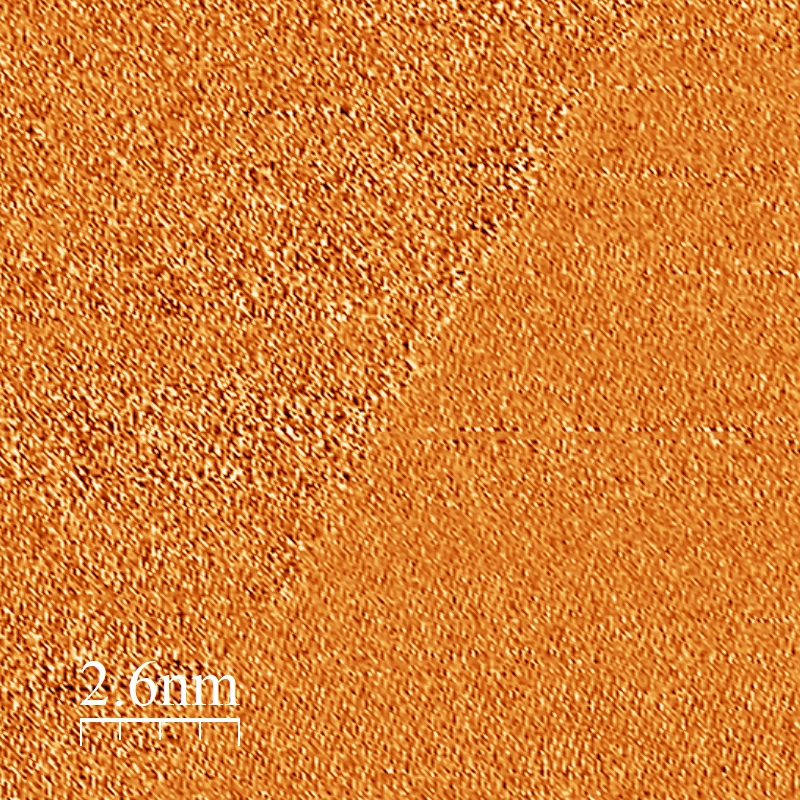
\includegraphics[scale=0.36]{Bilder/Igain8000_Strom.jpg}
\caption{Veranschaulichung der Effekte eines niedrigen IGains im Höhenbild der Breite 13.2nm. \textbf{Links:} IGain von 4000.  \textbf{Rechts:} IGain von 8000. Darunter befinden sich die dazugehörigen Strombilder. Es ist deutlich zu sehen, dass das Bild unschärfer wird und die Anzahl an Fehllinien zunimmt.}
\label{fig:hoch2_h}
\end{figure}

\subsubsection{Vermessung einer Kante}
\begin{figure}
\centering
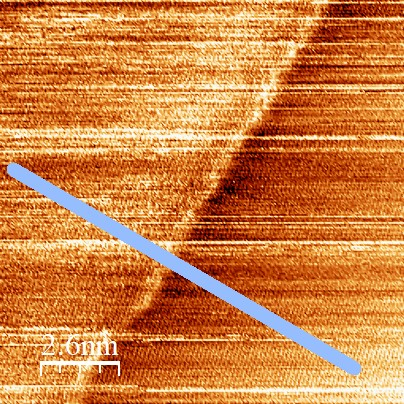
\includegraphics[scale=0.6]{Bilder/Anhang/Kante/0132_Kante_vor.jpg}
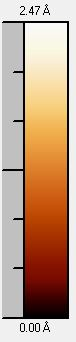
\includegraphics[scale=0.6]{Bilder/Anhang/Kante/0132_Kante_vor_Skala.jpg}
\caption{Bild der z-Komponente bei Vermessung der HOPG-Kante in einer Auflösung von (\SI{13,2}{nm})$^2$ in der Vorwärtsrichtung. Der breite Balken markiert die Stelle, an dem das Höhenprofil entnommen wurde.}
\label{fig:Kante_Beispiel}
\end{figure}

\begin{table}
\centering
\begin{tabular}{|c|c|c|c|c|c|}
\hline 
Auflösung & Messrichtung & Steigung & Achsenabschnitt [nm] & $\chi ^2$/ndof \\ 
\hline 
$(\SI{13,2}{nm})^2$ & Vorwärts & 0,109 $\pm$ 0,012 & 0,833 $\pm$ 0,041 & 12,550 \\
\hline 
$(\SI{13,2}{nm})^2$ & Rückwärts & 0,184 $\pm$ 0,012 & 0,414 $\pm$ 0,039 & 10,576\\
\hline 
$(\SI{29,7}{nm})^2$ & Vorwärts & 0,017 $\pm$ 0,011 & 1,019 $\pm$ 0,042 & 6,735 \\
\hline 
$(\SI{29,7}{nm})^2$ & Rückwärts & 0,043 $\pm$ 0,012 & 0,749 $\pm$ 0,045 & 7,726\\
\hline 
$(\SI{64,4}{nm})^2$ & Vorwärts & 0,034 $\pm$ 0,003 & 1,928 $\pm$ 0,032 & 5,626 \\
\hline 
$(\SI{64,4}{nm})^2$ & Rückwärts & 0,035 $\pm$ 0,001 & 1,498 $\pm$ 0,018 & 1,852\\
\hline 
$(\SI{126,9}{nm})^2$ & Vorwärts & 0,037 $\pm$ 0,001 & 1,936 $\pm$ 0,017 & 1,341 \\
\hline 
$(\SI{126,9}{nm})^2$ & Rückwärts & 0,017 $\pm$ 0,002 & 2,314 $\pm$ 0,030 & 2,969\\
\hline
\end{tabular} 
\caption{Ergebnisse der linearen Regressionen an Daten vor der Kante.}
\label{tab:Kante_linreg_vor_Ergebnisse}
\end{table}

\begin{table}
\centering
\begin{tabular}{|c|c|c|c|c|c|}
\hline 
Auflösung & Messrichtung & Steigung & Achsenabschnitt [nm] & $\chi ^2$/ndof \\ 
\hline 
$(\SI{13,2}{nm})^2$ & Vorwärts & 0,215 $\pm$ 0,006 & -1,178 $\pm$ 0,055 & 3,187 \\
\hline 
$(\SI{13,2}{nm})^2$ & Rückwärts & 0,172 $\pm$ 0,005 & -1,024 $\pm$ 0,050 & 3,323\\
\hline 
$(\SI{29,7}{nm})^2$ & Vorwärts & 0,033 $\pm$ 0,012 & -0,022 $\pm$ 0,124 & 2,672  \\
\hline 
$(\SI{29,7}{nm})^2$ & Rückwärts & 0,011 $\pm$ 0,009 & 0,147 $\pm$ 0,098 & 1,813\\
\hline 
$(\SI{64,4}{nm})^2$ & Vorwärts & -0,004 $\pm$ 0,004 & 0,527 $\pm$ 0,124 & 3,124\\
\hline 
$(\SI{64,4}{nm})^2$ & Rückwärts & 0,001 $\pm$ 0,003 & 0,250 $\pm$ 0,101 & 3,324\\
\hline 
$(\SI{126,9}{nm})^2$ & Vorwärts & 0,033 $\pm$ 0,008 & -1,488 $\pm$ 0,435 & 6,826\\
\hline 
$(\SI{126,9}{nm})^2$ & Rückwärts & 0,031 $\pm$ 0,002 & -1,157 $\pm$ 0,121 & 3,413\\
\hline 
\end{tabular} 
\caption{Ergebnisse der linearen Regressionen an Daten hinter der Kante.}
\label{tab:Kante_linreg_nach_Ergebnisse}
\end{table}

\begin{table}
\centering
\begin{tabular}{|c|c|c|c|c|}
\hline 
Auflösung & Messrichtung & $x_k$ [nm] & $y_k$ [nm] \\ 
\hline 
$(\SI{13,2}{nm})^2$ & Vorwärts & 6,16 & 0,72 \\
\hline 
$(\SI{13,2}{nm})^2$ & Rückwärts & 5,91 & 0,74 \\
\hline 
$(\SI{29,7}{nm})^2$ & Vorwärts & 7,69 & 0,73 \\
\hline 
$(\SI{29,7}{nm})^2$ & Rückwärts & 6,98 & 0,75 \\
\hline 
$(\SI{64,4}{nm})^2$ & Vorwärts & 25,22 & 0,97 \\
\hline 
$(\SI{64,4}{nm})^2$ & Rückwärts & 23,19 & 0,93 \\
\hline 
$(\SI{126,9}{nm})^2$ & Vorwärts & 34,24 & 1,80 \\
\hline 
$(\SI{126,9}{nm})^2$ & Rückwärts & 25,95 & 1,47 \\
\hline 
\end{tabular} 
\caption{Abgelesene Kantenmittelpunkte.}
\label{tab:Kantenmittelpunkte_Ergebnisse}
\end{table}

Auch bei der Vermessung der Kante wird ein Höhenprofil entnommen. Dabei muss darauf geachtet werden, dass das Höhenprofil möglichst senkrecht auf der Kante steht. Abbildung \ref{fig:Kante_Beispiel} zeigt dies beispielhaft für die Messung mit einem Messbereich von (\SI{13,2}{nm})$^2$.\\
Zur Bestimmung der Kantenhöhe wird an den Bereich vor und hinter der Kante jeweils eine Gerade angepasst und deren Abstand bestimmt. Dieser Abstand wird bestimmt, indem eine Gerade konstruiert wird, die senkrecht auf der tiefer liegenden Gerade steht und durch den abgelesenen Mittelpunkt der Kante geht. Der Mittelpunkt der Kante hat nur eine sehr kleine Auswirkung auf die Höhe, daher wird der Fehler auf diesen vernachlässigt. Um die Auswertung zu vereinfachen wurde hierfür ein realer Datenpunkt verwendet. Damit bestimmt sich die Geradengleichung dieser Gerade zu:
\begin{equation*}
y = \dfrac{-1}{a_{hinter}} \cdot x + y_k + \dfrac{x_k}{a_{hinter}}
\end{equation*}
Wobei $(x_k, y_k)$ die Koordinaten des abgelesenen Kantenmittelpunktes und $a_{hinter}$ die Steigung der angepassten Gerade hinter der Kante sind. Dann werden die Schnittpunkte dieser Geraden mit denen vor bzw. hinter der Kante bestimmt. Mit diesen Schnittpunkten ergibt sich die Höhe der Kante zu:
\begin{equation*}
h = \sqrt{(\Delta x)^2 + (\Delta y)^2}
\end{equation*}

\begin{figure}
\centering
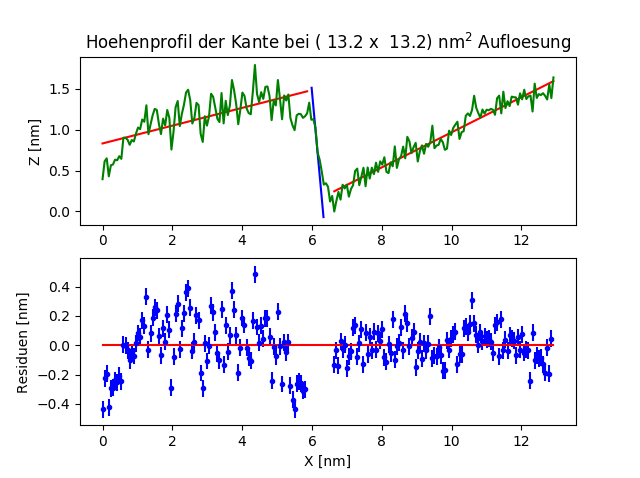
\includegraphics[scale=0.6]{Bilder/Anhang/Kante/Profil_Kante_0132_vor.png}
\caption{Entnommenes Höhenprofil (grün), angepasste Geraden (rot) und Kantengerade (orange) bei Vermessung der HOPG-Kante in einer Auflösung von (\SI{13,2}{nm})$^2$ in der Vorwärtsrichtung. In gelb sind die Verschiebungen der angepassten Geraden eingezeichnet, die die maximale Höhe ergeben haben, und in blau die, die die minimale Höhe ergeben haben. Die Residuen beziehen sich auf die vor bzw. hinter der Kante angepassten Geraden.}
\label{fig:Kante_Hoehenprofil_Beispiel}
\end{figure}

Für die Fehlerabschätzung werden Steigung und Achsenabschnitt der angepassten Geraden  um ihre Fehler variiert und mit jeder Variation die Kantenhöhe erneut ausgerechnet. Damit ergibt sich ein Bereich um den berechneten Wert, der den Fehler begrenzt. Die Werte für die Kantenhöhe mit ihren Fehlern sind in Tabelle \ref{tab:Kantenhöhe_Ergebnisse} dargestellt.\\
Abbildung \ref{fig:Kante_Hoehenprofil_Beispiel} zeigt das Höhenprofil, die angepassten und verschobenen Geraden und die Kantengerade für die in Abbildung \ref{fig:Kante_Beispiel} gezeigte Messung.

\begin{table}
\centering
\begin{tabular}{|c|c|c|}
\hline 
Auflösung & Messrichtung & Höhe [nm]\\ 
\hline 
$(\SI{13,2}{nm})^2$ & Vorwärts & $1,35 \pm 0,20$\\
\hline 
$(\SI{13,2}{nm})^2$ & Rückwärts & $1,49 \pm 0,19$\\
\hline 
$(\SI{29,7}{nm})^2$ & Vorwärts & $0,92 \pm 0,34$\\
\hline 
$(\SI{29,7}{nm})^2$ & Rückwärts & $0,83 \pm 0,29$\\
\hline 
$(\SI{64,4}{nm})^2$ & Vorwärts & $2,36 \pm 0,31$\\
\hline 
$(\SI{64,4}{nm})^2$ & Rückwärts & $2,02\pm 0,23$\\
\hline 
$(\SI{126,9}{nm})^2$ & Vorwärts & $3,58 \pm 0,76$\\
\hline 
$(\SI{126,9}{nm})^2$ & Rückwärts & $3,08 \pm 0,27$\\
\hline
\end{tabular} 
\caption{Ergebnisse für die Kantenhöhe.}
\label{tab:Kantenhöhe_Ergebnisse}
\end{table}

\begin{table}
\centering
\begin{tabular}{|c|c|c|}
\hline 
Auflösung & Höhe [nm] & Anzahl Netzebenen\\ 
\hline 
$(\SI{13,2}{nm})^2$ & $1,42 \pm 0,14$ & 4 \\
\hline 
$(\SI{29,7}{nm})^2$ & $0,87 \pm 0,22$ & 2-3 \\
\hline 
$(\SI{64,4}{nm})^2$ & $2,14 \pm 0,18$ & 6 \\
\hline 
$(\SI{126,9}{nm})^2$ & $3,14 \pm 0,25$ & 9-10 \\
\hline
\end{tabular} 
\caption{Gewichtet gemittelte Kantenhöhen und Anzahl der Netzebenen, die den Kantenhöhen entsprechen.}
\label{tab:Kantenhöhe_EndErgebnisse}
\end{table}

Die Werte für die Kantenhöhe stimmen für dasselbe Bild in Vor- und Rückrichtung jeweils innerhalb ihrer Fehler überein, daher können die Kantenhöhen der Richtungen gewichtet gemittelt werden (siehe Tabelle \ref{tab:Kantenhöhe_EndErgebnisse}). Allerdings wurde nicht auf jedem Bild die gleiche Stelle der Kante vermessen, sodass die Höhe von Bild zu Bild variiert. Mit der Literaturangabe für den Netzebenenabstand von \SI{335}{pm} lässt sich nun die Zahl der Netzebenen bestimmen, die die vermessene Kante verursachen (ebenfalls in Tabelle \ref{tab:Kantenhöhe_EndErgebnisse}). Die Fehler auf die gewichteten Mittelwerte sind dabei kleiner als ein Netzebenenabstand. Da diese Kantenhöhen nur ganzzahlige Vielfache des Netzebenenabstandes sein können, kann die Kantenhöhe auf 1 Netzebenenabstand genau bestimmt werden.

\subsubsection{Kalibration der Achsen}

\begin{figure}
\centering
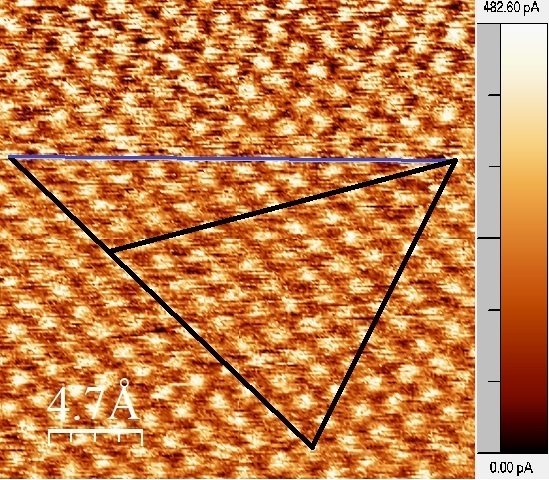
\includegraphics[scale=0.8]{Bilder/Atome/hoch2_h_scale.jpg}
\caption{Methode zur Bestimmung der x-Korrektur gezeigt am Bild im Konstanthöhenmodus mit einer Rastergröße von 2.325nm. Die blaue Linie gibt die zu bestimmende Länge an}
\label{fig:hoch2_h}
\end{figure}

\begin{figure}
\centering
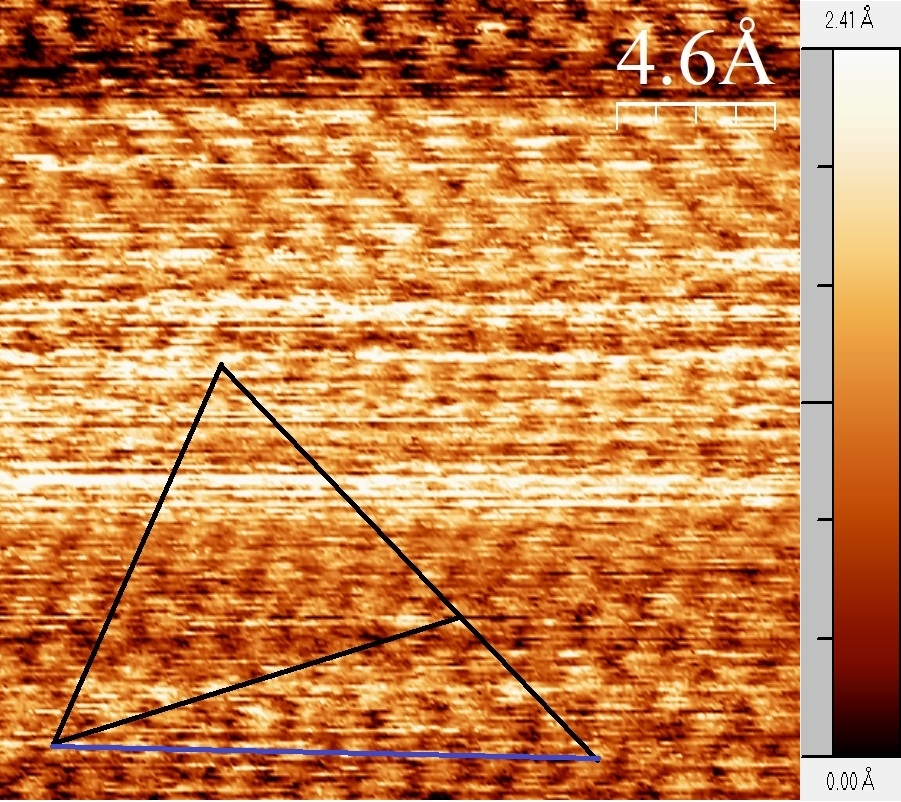
\includegraphics[scale=0.5]{Bilder/Atome/strom2_h_scale.jpg}
\caption{Methode zur Bestimmung der x-Korrektur gezeigt am Bild im Konstantstrommodus mit einer Rastergröße von 2.325nm. Die blaue Linie gibt die zu bestimmende Länge an}
\label{fig:strom2_h}
\end{figure}

Um die Längenskalen in x- und y-Richtung möglichst unkorreliert kalibrieren zu können, kann nicht direkt der Atomabstand benutzt werden. Stattdessen wird der Abstand zwischen 2 Atomen bestimmt, die möglichst auf einer der beiden Achsen liegen. Dann wird über ein Dreieck entlang der Symmetrieachsen des Atomgitters die echte Länge dieses Abstandes bestimmt.\\
Dies ist möglich, da man aus der Gitterstruktur den Winkel zwischen den Symmetrieachsen($60^{\circ}$) und die Atomabstände (\SI{2.46}{\angstrom}) und damit die Längen entlang der Achsen kennt. Man kann also die Atome entlang des Dreieckes zählen daraus über den Kosinussatz die Länge in die Achsenrichtung bestimmen:
\begin{equation}
c = \sqrt{(a\cdot n)^{2}+(a\cdot m)^2-2 a^{2}\cdot n\cdot m\cdot cos(\alpha)}
\end{equation}
Hierbei ist c die zu bestimmende Länge, a die Atomlänge, n und m die Anzahl der Atome entlang einer Dreiecksseite und $\alpha$ der Winkel zwischen diesen Seiten.\\Da kein Fehler auf den Atomabstand angenommen wird, ist dieser Wert exakt.
In Abbildung \ref{fig:hoch2_h} und \ref{fig:strom2_h} ist diese Methode beispielhaft anhand den 2.325nm Messungen gezeigt.\\
Vor allem bei größeren Rasterbereichen konnte oft die Anzahl der Atome nicht mit 100\% Genauigkeit bestimmt werden.
Um mögliche Zählfehler erkennen zu können wurde deswegen sowohl einmal über die  $60^{\circ}$-Symmetrie, als auch einmal über $120^{\circ}$-Symmetrie die Länge bestimmt. Diese Längen sollten identisch sein. Wenn dies nicht der Fall ist, hat man sich offensichtlich verzählt.\\
Die Atome waren manchmal sehr schwer zu erkennen, weswegen stattdessen die Anzahl oft anhand der durchquerten Symmetrieachsen bestimmt wurde. Dies ist schematisch in Abbildung \ref{fig:strom5_symmetire} dargestellt.\\
\\
Es muss außerdem noch die gemessene Länge von c im Bild bestimmt werden.\\
Dazu wird an insgesamt 6 verschiedenen Stellen der Abstand zwischen zwei Atomen gemessen, die die gleiche Anzahl von Atomen zwischen sich liegen haben.
Dies ist ebenfalls schematisch in Abbildung \ref{fig:strom2_abstand} dargestellt.\\
Die so erhaltenden Längen wurden gemittelt. Daraus erhält man auch einen Fehler auf die Längen, welcher die Ableseungenauigkeit der Atompositionen und mögliche Schwankungen der Atomabstände berücksichtigt.
\\
Mit diesem Verfahren wurden alle 6 Messungen jeweils unabhängig für die x- und y-Richtung ausgewertet. Die Ergebnisse sind in Tabelle \ref{tab:Atome_horizontal} für die x-Richtung und in Tabelle \ref{tab:Atome_vertikal} für die y-Richtung zusammengefasst.\\
Die restlichen Bilder, die zur Auswertung benutzt wurden, befinden sich im Anhang.\\


\begin{figure}
\centering
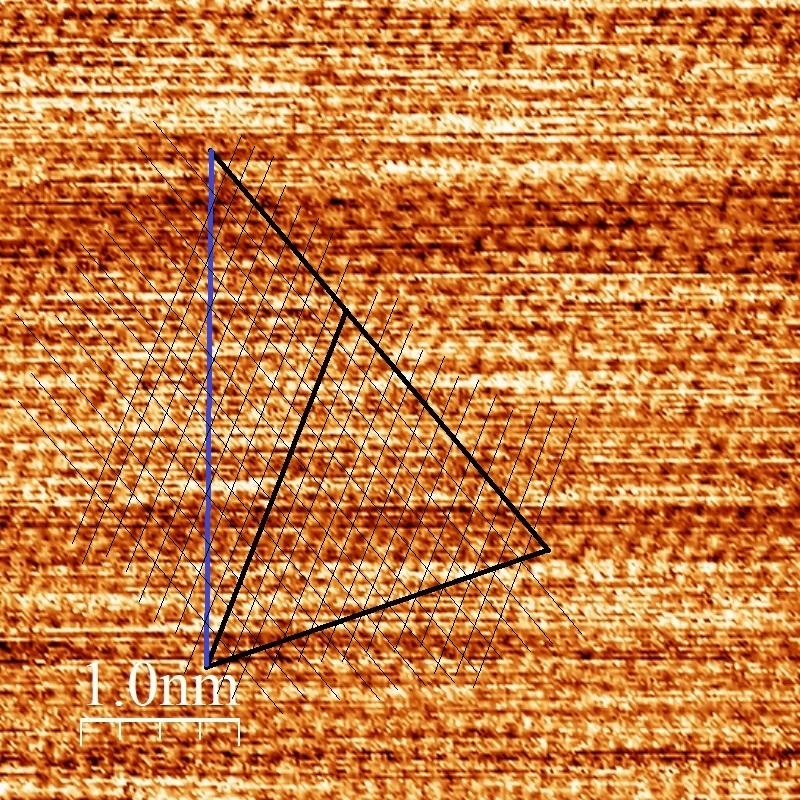
\includegraphics[scale=0.6]{Bilder/Atome/strom5_v_gitter.jpg}
\caption{Darstellung des sichtbaren Atomgitters anhand der 5nm Strommessung, um das Ablesen der Atomanzahl zu vereinfachen.}
\label{fig:strom5_symmetire}
\end{figure}

\begin{figure}
\centering
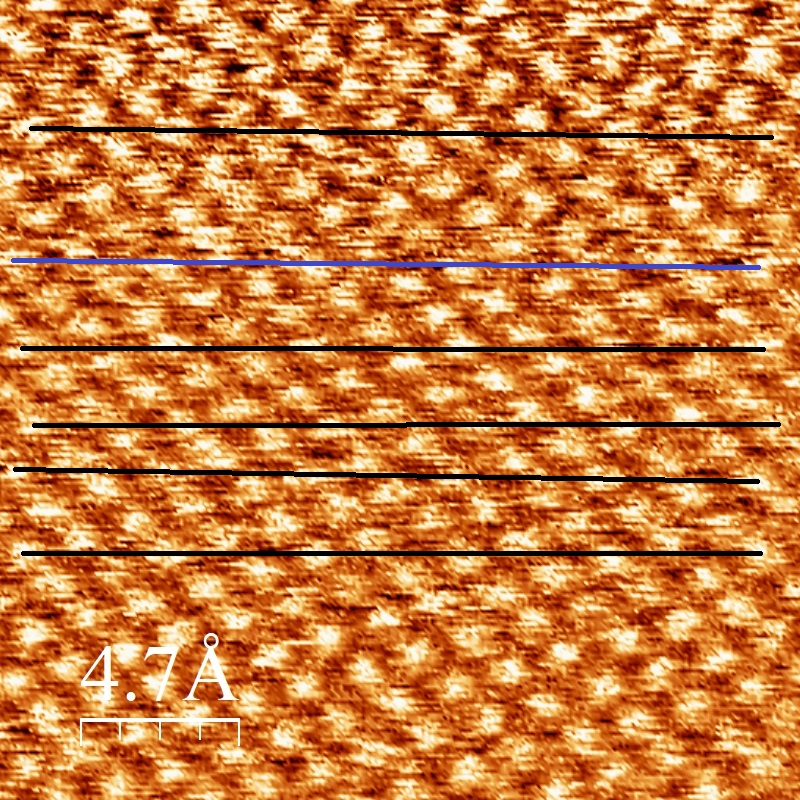
\includegraphics[scale=0.54]{Bilder/Atome/hoch2_abstand.jpg}
\caption{Beispielhafte Auswahl von 6 Abständen, die den Originalabstand(blau) repräsentieren. Die Abstände wurden gemittelt, um die gemessene Länge bestimmen zu können.}
\label{fig:strom2_abstand}
\end{figure}


\begin{table}
\begin{tabular}{|c|c|c||c|c||c|c|}
\hline 
Modus & Bildbreite [\si{\angstrom}] & Abstand [\si{\angstrom}] & Atome($60^{\circ}$) & Atome($120^{\circ}$) & ber. Länge [\si{\angstrom}] & rel. Länge\\ 
\hline 
\hline 
Höhen & 10 & $8.81\pm 0.04$ & 6/4 & 2/4 & 13.02& $0.677\pm 0.003$\\ 
\hline 
Höhen & 23.25 & $21.50\pm 0.04$ & 10/15 & 10/5 & 32.54& $0.661\pm 0.001$\\ 
\hline 
Höhen & 50 & $18.4\pm 0.07$ & 4/6  & 4/2 & 28.38& $0.648\pm 0.002$\\ 
\hline 
\hline
Strom & 8.719 & $6.07\pm 0.03$ & 4/6 & 4/2 & 8.87& $0.684\pm 0.003$\\ 
\hline 
Strom & 23.25 & $16.74\pm 0.14$ & 7/11  & 7/4 & 23.72& $0.706\pm 0.006$\\ 
\hline 
Strom & 50 & $40.00\pm 0.09$ & 19/28  & 19/9 & 60.91& $0.657\pm 0.001$\\ 
\hline 
\end{tabular} 
\caption{Ergebnisse der \textbf{horizontalen} Längenmessung. Angegeben ist der verwendete Modus(Konstanthöhen-/Konstantstrommodus), die Bildbreite, der abgelesene Abstand, die Anzahl der Atome über einen $60^{\circ}$/$120^{\circ}$ Winkel, die daraus berechnete Länge und das Verhältnis von abgelesener zur berechneten Länge.}
\label{tab:Atome_horizontal}
\end{table}

\begin{table}
\begin{tabular}{|c|c|c||c|c||c|c|}
\hline 
Modus & Bildbreite [\si{\angstrom}]  & Abstand [\si{\angstrom}] & Atome($60^{\circ}$) & Atome($120^{\circ}$) & ber. Länge [\si{\angstrom}] & rel. Länge\\ 
\hline 
\hline 
Höhen & 10 & $8.55\pm 0.04$ & 5/4 & 5/9 & 19.21& $0.445\pm 0.002$\\ 
\hline 
Höhen & 23.25 & $20.81\pm 0.06$ & 10/17  & 10/7 & 36.40& $0.572\pm 0.002$\\ 
\hline 
Höhen & 50 & $22.88\pm 0.17$ & 10/17  & 10/7 & 36.40& $0.629\pm 0.005$\\ 
\hline 
\hline 
Strom & 8.719 & $6.18\pm 0.06$ & 3/2 & 3/5 & 10.72& $0.576\pm 0.006$\\
\hline 
Strom & 23.25 & $18.00\pm 0.07$ & 8/14  & 8/6 & 29.93& $0.601\pm 0.002$\\
\hline 
Strom & 50 & $32.22\pm 0.15$ & 13/22  & 13/9 & 47.13& $0.684\pm 0.003$\\
\hline 
\end{tabular} 
\caption{Ergebnisse der \textbf{vertikalen} Längenmessung. Angegeben ist der verwendete Modus(Konstanthöhen-/Konstantstrommodus), die Bildbreite, der abgelesene Abstand, die Anzahl der Atome über einen $60^{\circ}$/$120^{\circ}$ Winkel, die daraus berechnete Länge und das Verhältnis von abgelesener zur berechneten Länge.}
\label{tab:Atome_vertikal}
\end{table}

Es ist auffällig, dass die vertikalen Korrekturfaktoren mit zunehmender Bereichsgröße anwachsen, die berechnete Strecke also besser mit der gemessenen übereinstimmt. Dies kann an Drift- und Creep-Effekten liegen. Bei kleineren Bildgrößen wird der Piezokristall weniger bewegt. Dadurch haben die Nebeneffekte, deren Größe sich nicht unbedingt mit der Bewegungsweite ändert, einen größeren relativen Einfluss und verschieben die Atome mehr, wodurch die gemessene Strecke mehr von der ausgerechneten abweicht.\\
Diese Effekte treten in horizontaler Richtung nicht auf, da dort der Kristall sehr viel schneller weiterbewegt wird.\\
Diese Effekte sorgen dafür, dass die Korrekturfaktoren von verschiedenen Bildern nicht unbedingt innerhalb ihrer Fehler übereinstimmen.

Eine gewichtete Mittelung (mit äußerem Fehler) der Korrekturfaktoren, also dem Verhältnis von der berechneten Länge im Bild zur "echten" berechneten Länge, ergibt das Endergebnis:
\begin{equation*}
\boxed{\textrm{horizontale Korrektur}: 0.660\pm 0.004}
\end{equation*}

\begin{equation*}
\boxed{\textrm{vertikale Korrektur}: 0.561\pm 0.035}
\end{equation*}


\section{Fazit}
Bei der Untersuchung der Mikroskopeigenschaften haben sich ein I-Gain von 3000 und eine Messzeit pro Zeile von \SI{600}{ms} als ideal herausgestellt, da Flanken bei Vermessung in beiden Richtungen gleich dargestellt werden bzw. die gemessenen Flankensteigungen innerhalb ihrer Fehler übereinstimmen.\\
Bei höherem IGain nimmt die Schwankung der Daten sowohl im z-Bild, als auch im Höhenbild deutlich zu, was mit der Erwartung des Überschwingens übereinstimmt.\\
Der Einfluss der Messzeit auf das Messergebnis spielt eine eher kleine Rolle. Wichtig ist vor allem, dass diese zum I-Gain passt, da I-Gain und Messzeit pro Zeile (quasi die Messgeschwindigkeit) festlegen, welcher räumliche Bereich zur Regelung beiträgt, was nach der zeitlichen Regelung der zweitgrößte Effekt ist, der ein Überschwingen des Probe-Spitze-Abstandes verursachen kann. \\
\\
Die Höhe der vermessenen Kante konnte mit kleinen Fehlern ($\sigma _h < d_{Netzebenen}$) bestimmt werden, sodass innerhalb des Fehlers um den gemessenen Wert herum maximal zwei ganzzahlige Vielfache des Netzebenenabstandes $d_{Netzebenen}$ liegen. Zudem gab es keinen Wert, der innerhalb des Fehlers nicht mit einem ganzzahligen Vielfachen übereinstimmte. Die Höhen der vermessenen Kante waren in den unterschiedlichen Zoom-Stufen jedoch unterschiedlich groß. Es handelt sich zwar um dieselbe Kante, jedoch sind die Höhenprofile nicht alle an der gleichen Stelle entnommen, sodass davon ausgegangen werden kann, dass die vermessene Kante nicht gleichmäßig hoch ist.\\
\\
Anhand der Atomabstände konnten die horizontalen und vertikalen Rasterlängen kalibriert werden. Es ergeben sich Korrekturfakturen von $0.561\pm 0.035$ in vertikaler und $0.660\pm 0.004$ in horizontaler Richtung. In vertikaler Richtung spielen dabei Nebeneffekte wie thermischer Drift und Creep bei kleineren Rasterbereichen eine immer größer werdende Rolle.


\newpage
\section{Anhang}
\subsection{Goldproben}
\subsubsection{I-Gain}
\begin{figure}[H]
\centering
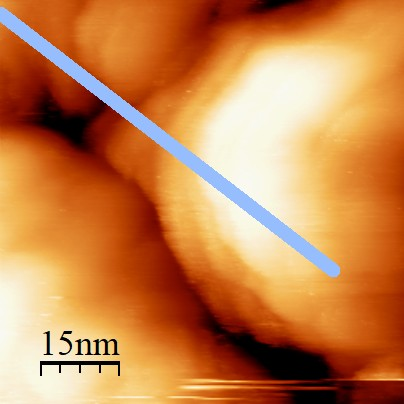
\includegraphics[scale=0.6]{Bilder/Anhang/IGain/1000_IGain_vor.jpg}
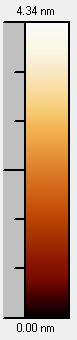
\includegraphics[scale=0.6]{Bilder/Anhang/IGain/1000_IGain_vor_Skala.jpg}
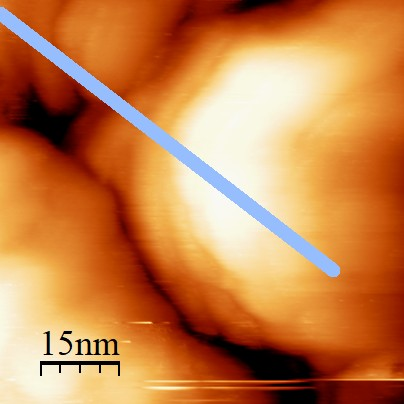
\includegraphics[scale=0.6]{Bilder/Anhang/IGain/1000_IGain_nach.jpg}
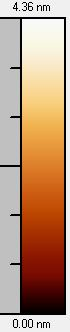
\includegraphics[scale=0.6]{Bilder/Anhang/IGain/1000_IGain_nach_Skala.jpg}
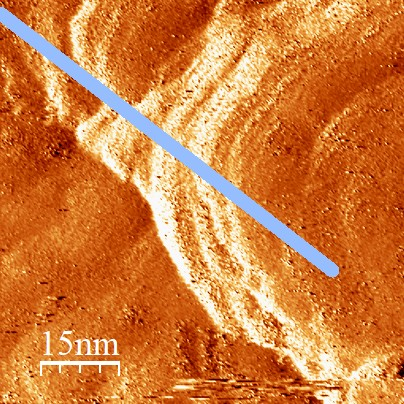
\includegraphics[scale=0.6]{Bilder/Anhang/IGain/Strom/1000_IGain_Strom_vor.jpg}
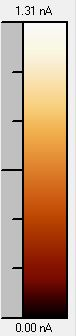
\includegraphics[scale=0.6]{Bilder/Anhang/IGain/Strom/1000_IGain_Strom_vor_Skala.jpg}
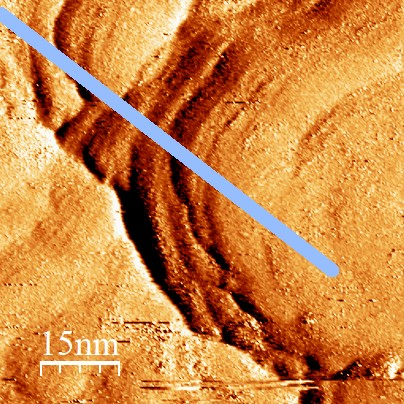
\includegraphics[scale=0.6]{Bilder/Anhang/IGain/Strom/1000_IGain_Strom_nach.jpg}
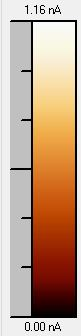
\includegraphics[scale=0.6]{Bilder/Anhang/IGain/Strom/1000_IGain_Strom_nach_Skala.jpg}
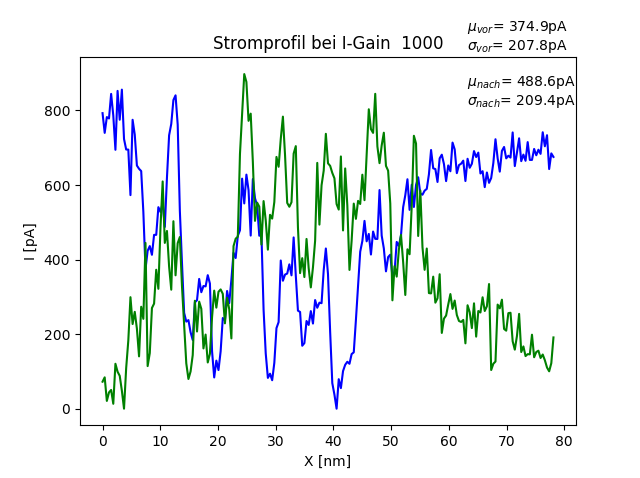
\includegraphics[scale=0.5]{Bilder/Anhang/IGain/Strom/Strom_Profil_IGain_1000.png}
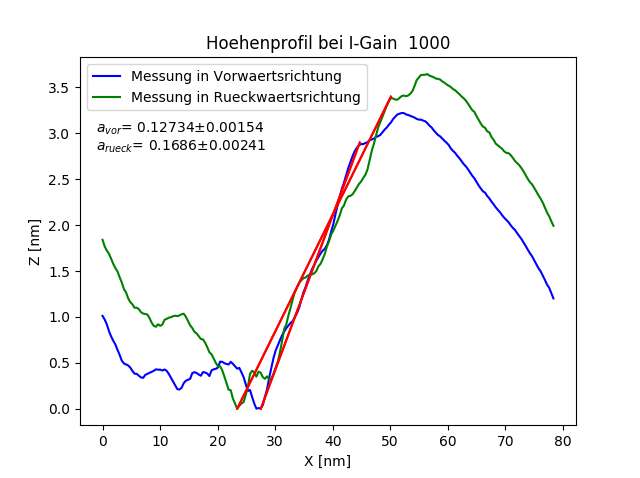
\includegraphics[scale=0.5]{Bilder/Anhang/IGain/Profil_IGain_1000.png}
\caption{\textbf{Oben}: Bild der z-Komponente bei Vermessung der Goldprobe mit einem I-Gain von 1000 in der Vorwärtsrichtung (rechts) und der Rückwärtsrichtung (links). \textbf{Mitte}: Zugehörige Bilder des Stroms \textbf{Unten}: Stromprofil (links) und entnommenes Höhenprofil und abgelesene Flanken (rechts).}
\end{figure}

\begin{figure}[H]
\centering
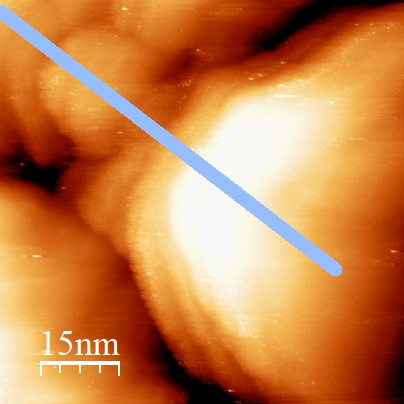
\includegraphics[scale=0.6]{Bilder/Anhang/IGain/3000_IGain_vor.jpg}
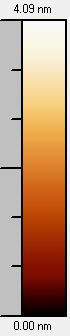
\includegraphics[scale=0.6]{Bilder/Anhang/IGain/3000_IGain_vor_Skala.jpg}
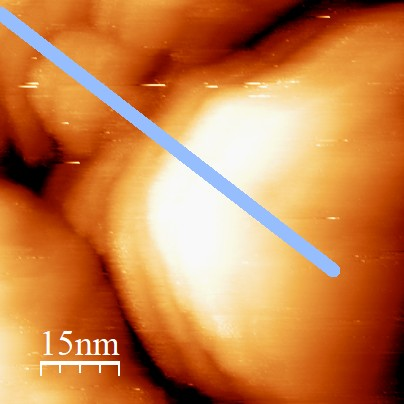
\includegraphics[scale=0.6]{Bilder/Anhang/IGain/3000_IGain_nach.jpg}
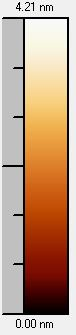
\includegraphics[scale=0.6]{Bilder/Anhang/IGain/3000_IGain_nach_Skala.jpg}
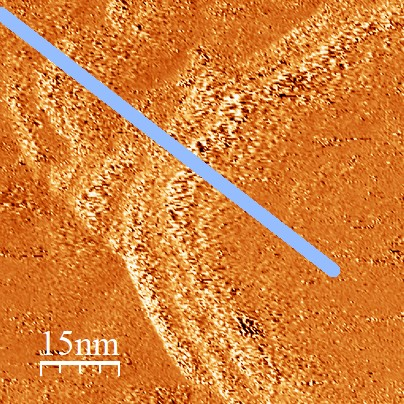
\includegraphics[scale=0.6]{Bilder/Anhang/IGain/Strom/3000_IGain_Strom_vor.jpg}
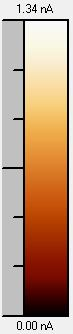
\includegraphics[scale=0.6]{Bilder/Anhang/IGain/Strom/3000_IGain_Strom_vor_Skala.jpg}
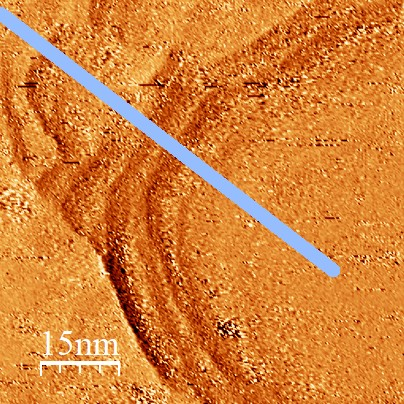
\includegraphics[scale=0.6]{Bilder/Anhang/IGain/Strom/3000_IGain_Strom_nach.jpg}
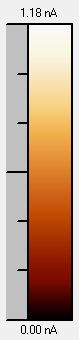
\includegraphics[scale=0.6]{Bilder/Anhang/IGain/Strom/3000_IGain_Strom_nach_Skala.jpg}
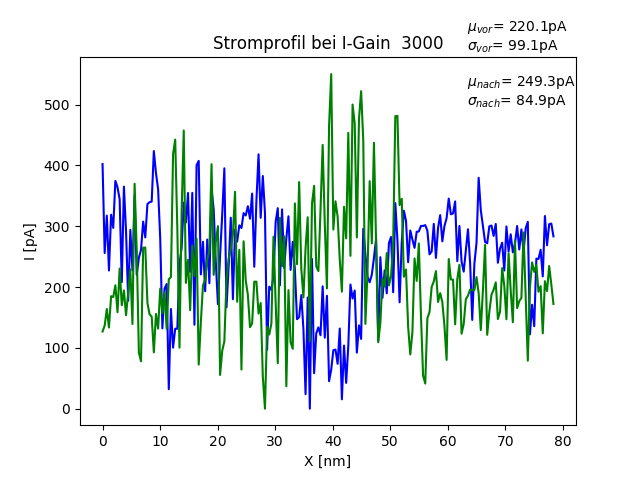
\includegraphics[scale=0.5]{Bilder/Anhang/IGain/Strom/Strom_Profil_IGain_3000.png}
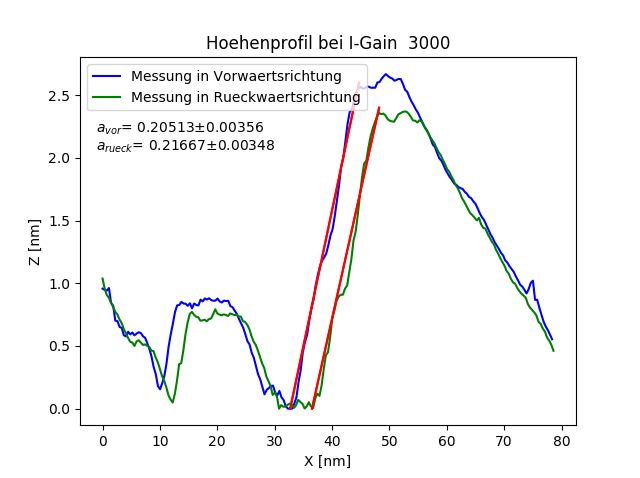
\includegraphics[scale=0.5]{Bilder/Anhang/IGain/Profil_IGain_3000.png}
\caption{\textbf{Oben}: Bild der z-Komponente bei Vermessung der Goldprobe mit einem I-Gain von 3000 in der Vorwärtsrichtung (rechts) und der Rückwärtsrichtung (links). \textbf{Mitte}: Zugehörige Bilder des Stroms \textbf{Unten}: Stromprofil (links) und entnommenes Höhenprofil und abgelesene Flanken (rechts).}
\end{figure}

\begin{figure}[H]
\centering
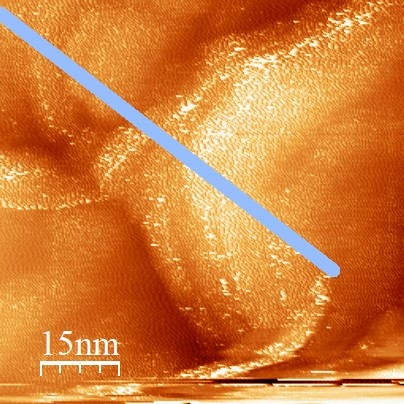
\includegraphics[scale=0.6]{Bilder/Anhang/IGain/8000_IGain_vor.jpg}
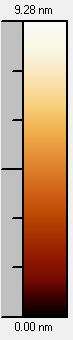
\includegraphics[scale=0.6]{Bilder/Anhang/IGain/8000_IGain_vor_Skala.jpg}
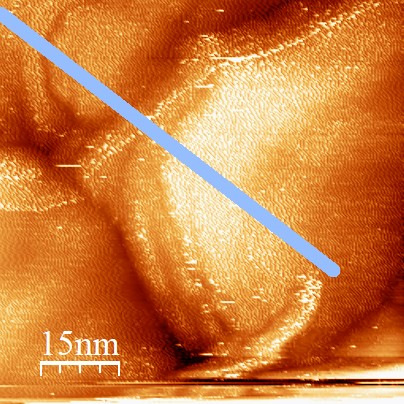
\includegraphics[scale=0.6]{Bilder/Anhang/IGain/8000_IGain_nach.jpg}
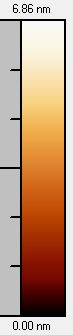
\includegraphics[scale=0.6]{Bilder/Anhang/IGain/8000_IGain_nach_Skala.jpg}
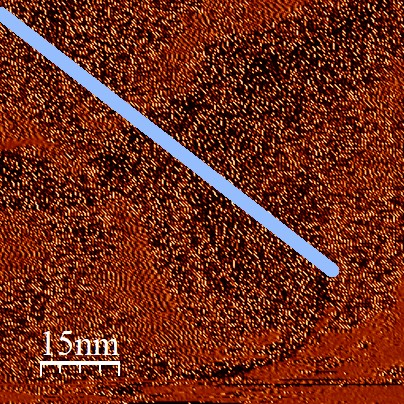
\includegraphics[scale=0.6]{Bilder/Anhang/IGain/Strom/8000_IGain_Strom_vor.jpg}
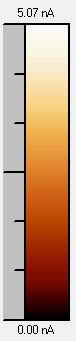
\includegraphics[scale=0.6]{Bilder/Anhang/IGain/Strom/8000_IGain_Strom_vor_Skala.jpg}
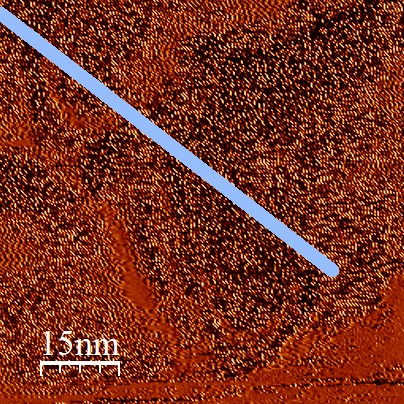
\includegraphics[scale=0.6]{Bilder/Anhang/IGain/Strom/8000_IGain_Strom_nach.jpg}
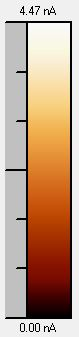
\includegraphics[scale=0.6]{Bilder/Anhang/IGain/Strom/8000_IGain_Strom_nach_Skala.jpg}
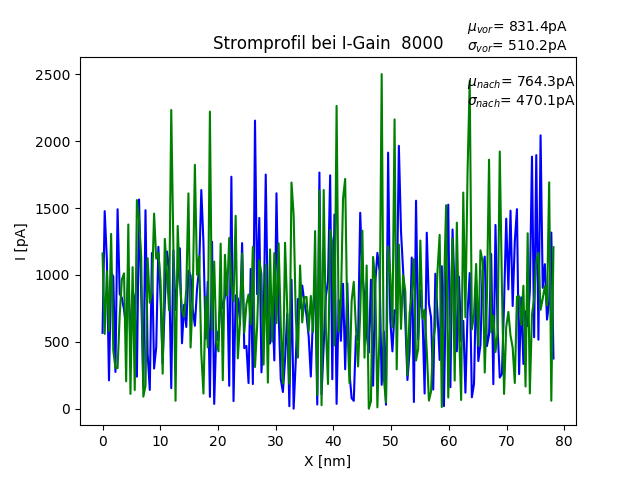
\includegraphics[scale=0.5]{Bilder/Anhang/IGain/Strom/Strom_Profil_IGain_8000.png}
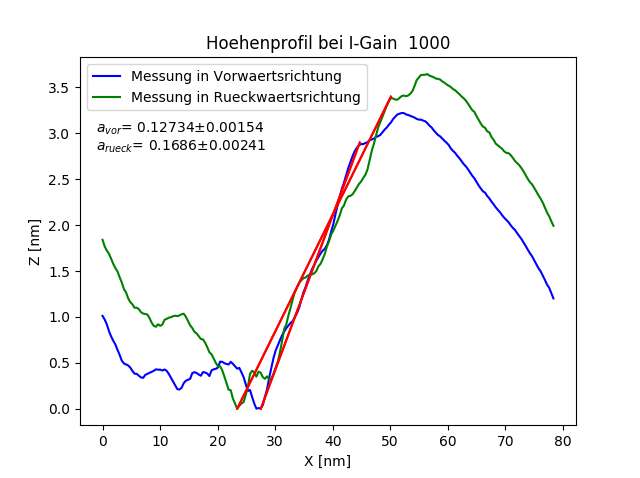
\includegraphics[scale=0.5]{Bilder/Anhang/IGain/Profil_IGain_1000.png}
\caption{\textbf{Oben}: Bild der z-Komponente bei Vermessung der Goldprobe mit einem I-Gain von 8000 in der Vorwärtsrichtung (rechts) und der Rückwärtsrichtung (links). \textbf{Mitte}: Zugehörige Bilder des Stroms \textbf{Unten}: Stromprofil (links) und entnommenes Höhenprofil und abgelesene Flanken (rechts).}
\end{figure}

\begin{figure}[H]
\centering
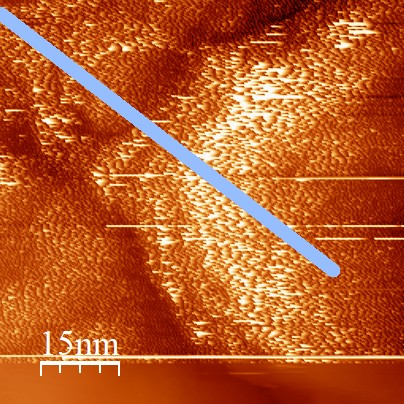
\includegraphics[scale=0.6]{Bilder/Anhang/IGain/11000_IGain_vor.jpg}
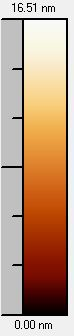
\includegraphics[scale=0.6]{Bilder/Anhang/IGain/11000_IGain_vor_Skala.jpg}
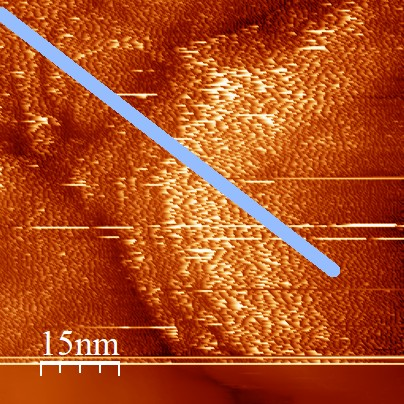
\includegraphics[scale=0.6]{Bilder/Anhang/IGain/11000_IGain_nach.jpg}
\includegraphics[scale=0.6]{Bilder/Anhang/IGain/11000_IGain_nach_Skala.jpg}
\includegraphics[scale=0.6]{Bilder/Anhang/IGain/Strom/11000_IGain_Strom_vor.jpg}
\includegraphics[scale=0.6]{Bilder/Anhang/IGain/Strom/11000_IGain_Strom_vor_Skala.jpg}
\includegraphics[scale=0.6]{Bilder/Anhang/IGain/Strom/11000_IGain_Strom_nach.jpg}
\includegraphics[scale=0.6]{Bilder/Anhang/IGain/Strom/11000_IGain_Strom_nach_Skala.jpg}
\includegraphics[scale=0.5]{Bilder/Anhang/IGain/Strom/Strom_Profil_IGain_11000.png}
\includegraphics[scale=0.5]{Bilder/Anhang/IGain/Profil_IGain_11000.png}
\caption{\textbf{Oben}: Bild der z-Komponente bei Vermessung der Goldprobe mit einem I-Gain von 11000 in der Vorwärtsrichtung (rechts) und der Rückwärtsrichtung (links). \textbf{Mitte}: Zugehörige Bilder des Stroms \textbf{Unten}: Stromprofil (links) und entnommenes Höhenprofil und abgelesene Flanken (rechts).}
\end{figure}

\subsubsection{Zeit}
\begin{figure}[H]
\centering
\includegraphics[scale=0.6]{Bilder/Anhang/Zeit/0_052_Zeit_vor.jpg}
\includegraphics[scale=0.6]{Bilder/Anhang/Zeit/0_052_Zeit_vor_Skala.jpg}
\includegraphics[scale=0.6]{Bilder/Anhang/Zeit/0_052_Zeit_nach.jpg}
\includegraphics[scale=0.6]{Bilder/Anhang/Zeit/0_052_Zeit_nach_Skala.jpg}
\includegraphics[scale=0.6]{Bilder/Anhang/Zeit/Strom/0_052_Zeit_vor_Strom.jpg}
\includegraphics[scale=0.6]{Bilder/Anhang/Zeit/Strom/0_052_Zeit_vor_Strom_Skala.jpg}
\includegraphics[scale=0.6]{Bilder/Anhang/Zeit/Strom/0_052_Zeit_nach_Strom.jpg}
\includegraphics[scale=0.6]{Bilder/Anhang/Zeit/Strom/0_052_Zeit_nach_Strom_Skala.jpg}
\includegraphics[scale=0.5]{Bilder/Anhang/Zeit/Strom/Strom_Profil_Zeit_0052.png}
\includegraphics[scale=0.5]{Bilder/Anhang/Zeit/Profil_Zeit_52.png}
\caption{\textbf{Oben}: Bild der z-Komponente bei Vermessung der Goldprobe mit einer Messzeit von \SI{52}{ms} in der Vorwärtsrichtung (rechts) und der Rückwärtsrichtung (links). \textbf{Mitte}: Zugehörige Bilder des Stroms \textbf{Unten}: Stromprofil (links) und entnommenes Höhenprofil und abgelesene Flanken (rechts).}
\end{figure}

\begin{figure}[H]
\centering
\includegraphics[scale=0.6]{Bilder/Anhang/Zeit/0_08_Zeit_vor.jpg}
\includegraphics[scale=0.6]{Bilder/Anhang/Zeit/0_08_Zeit_vor_Skala.jpg}
\includegraphics[scale=0.6]{Bilder/Anhang/Zeit/0_08_Zeit_nach.jpg}
\includegraphics[scale=0.6]{Bilder/Anhang/Zeit/0_08_Zeit_nach_Skala.jpg}
\includegraphics[scale=0.6]{Bilder/Anhang/Zeit/Strom/0_080_Zeit_vor_Strom.jpg}
\includegraphics[scale=0.6]{Bilder/Anhang/Zeit/Strom/0_080_Zeit_vor_Strom_Skala.jpg}
\includegraphics[scale=0.6]{Bilder/Anhang/Zeit/Strom/0_080_Zeit_nach_Strom.jpg}
\includegraphics[scale=0.6]{Bilder/Anhang/Zeit/Strom/0_080_Zeit_nach_Strom_Skala.jpg}
\includegraphics[scale=0.5]{Bilder/Anhang/Zeit/Strom/Strom_Profil_Zeit_0080.png}
\includegraphics[scale=0.5]{Bilder/Anhang/Zeit/Profil_Zeit_52.png}
\caption{\textbf{Oben}: Bild der z-Komponente bei Vermessung der Goldprobe mit einer Messzeit von \SI{80}{ms} in der Vorwärtsrichtung (rechts) und der Rückwärtsrichtung (links). \textbf{Mitte}: Zugehörige Bilder des Stroms \textbf{Unten}: Stromprofil (links) und entnommenes Höhenprofil und abgelesene Flanken (rechts).}
\end{figure}

\begin{figure}[H]
\centering
\includegraphics[scale=0.6]{Bilder/Anhang/Zeit/0_1_Zeit_vor.jpg}
\includegraphics[scale=0.6]{Bilder/Anhang/Zeit/0_1_Zeit_vor_Skala.jpg}
\includegraphics[scale=0.6]{Bilder/Anhang/Zeit/0_1_Zeit_nach.jpg}
\includegraphics[scale=0.6]{Bilder/Anhang/Zeit/0_1_Zeit_nach_Skala.jpg}
\includegraphics[scale=0.6]{Bilder/Anhang/Zeit/Strom/0_1_Zeit_vor_Strom.jpg}
\includegraphics[scale=0.6]{Bilder/Anhang/Zeit/Strom/0_1_Zeit_vor_Strom_Skala.jpg}
\includegraphics[scale=0.6]{Bilder/Anhang/Zeit/Strom/0_1_Zeit_nach_Strom.jpg}
\includegraphics[scale=0.6]{Bilder/Anhang/Zeit/Strom/0_1_Zeit_nach_Strom_Skala.jpg}
\includegraphics[scale=0.5]{Bilder/Anhang/Zeit/Strom/Strom_Profil_Zeit_0100.png}
\includegraphics[scale=0.5]{Bilder/Anhang/Zeit/Profil_Zeit_100.png}
\caption{\textbf{Oben}: Bild der z-Komponente bei Vermessung der Goldprobe mit einer Messzeit von \SI{100}{ms} in der Vorwärtsrichtung (rechts) und der Rückwärtsrichtung (links). \textbf{Mitte}: Zugehörige Bilder des Stroms \textbf{Unten}: Stromprofil (links) und entnommenes Höhenprofil und abgelesene Flanken (rechts).}
\end{figure}

\begin{figure}[H]
\centering
\includegraphics[scale=0.6]{Bilder/Anhang/Zeit/0_2_Zeit_vor.jpg}
\includegraphics[scale=0.6]{Bilder/Anhang/Zeit/0_2_Zeit_vor_Skala.jpg}
\includegraphics[scale=0.6]{Bilder/Anhang/Zeit/0_2_Zeit_nach.jpg}
\includegraphics[scale=0.6]{Bilder/Anhang/Zeit/0_2_Zeit_nach_Skala.jpg}
\includegraphics[scale=0.6]{Bilder/Anhang/Zeit/Strom/0_2_Zeit_vor_Strom.jpg}
\includegraphics[scale=0.6]{Bilder/Anhang/Zeit/Strom/0_2_Zeit_vor_Strom_Skala.jpg}
\includegraphics[scale=0.6]{Bilder/Anhang/Zeit/Strom/0_2_Zeit_nach_Strom.jpg}
\includegraphics[scale=0.6]{Bilder/Anhang/Zeit/Strom/0_2_Zeit_nach_Strom_Skala.jpg}
\includegraphics[scale=0.5]{Bilder/Anhang/Zeit/Strom/Strom_Profil_Zeit_0200.png}
\includegraphics[scale=0.5]{Bilder/Anhang/Zeit/Profil_Zeit_200.png}
\caption{\textbf{Oben}: Bild der z-Komponente bei Vermessung der Goldprobe mit einer Messzeit von \SI{200}{ms} in der Vorwärtsrichtung (rechts) und der Rückwärtsrichtung (links). \textbf{Mitte}: Zugehörige Bilder des Stroms \textbf{Unten}: Stromprofil (links) und entnommenes Höhenprofil und abgelesene Flanken (rechts).}
\end{figure}

\begin{figure}[H]
\centering
\includegraphics[scale=0.6]{Bilder/Anhang/Zeit/0_4_Zeit_vor.jpg}
\includegraphics[scale=0.6]{Bilder/Anhang/Zeit/0_4_Zeit_vor_Skala.jpg}
\includegraphics[scale=0.6]{Bilder/Anhang/Zeit/0_4_Zeit_nach.jpg}
\includegraphics[scale=0.6]{Bilder/Anhang/Zeit/0_4_Zeit_nach_Skala.jpg}
\includegraphics[scale=0.6]{Bilder/Anhang/Zeit/Strom/0_4_Zeit_vor_Strom.jpg}
\includegraphics[scale=0.6]{Bilder/Anhang/Zeit/Strom/0_4_Zeit_vor_Strom_Skala.jpg}
\includegraphics[scale=0.6]{Bilder/Anhang/Zeit/Strom/0_4_Zeit_nach_Strom.jpg}
\includegraphics[scale=0.6]{Bilder/Anhang/Zeit/Strom/0_4_Zeit_nach_Strom_Skala.jpg}
\includegraphics[scale=0.5]{Bilder/Anhang/Zeit/Strom/Strom_Profil_Zeit_0400.png}
\includegraphics[scale=0.5]{Bilder/Anhang/Zeit/Profil_Zeit_400.png}
\caption{\textbf{Oben}: Bild der z-Komponente bei Vermessung der Goldprobe mit einer Messzeit von \SI{400}{ms} in der Vorwärtsrichtung (rechts) und der Rückwärtsrichtung (links). \textbf{Mitte}: Zugehörige Bilder des Stroms \textbf{Unten}: Stromprofil (links) und entnommenes Höhenprofil und abgelesene Flanken (rechts).}
\end{figure}

\begin{figure}[H]
\centering
\includegraphics[scale=0.6]{Bilder/Anhang/Zeit/0_6_Zeit_vor.jpg}
\includegraphics[scale=0.6]{Bilder/Anhang/Zeit/0_6_Zeit_vor_Skala.jpg}
\includegraphics[scale=0.6]{Bilder/Anhang/Zeit/0_6_Zeit_nach.jpg}
\includegraphics[scale=0.6]{Bilder/Anhang/Zeit/0_6_Zeit_nach_Skala.jpg}
\includegraphics[scale=0.6]{Bilder/Anhang/Zeit/Strom/0_6_Zeit_vor_Strom.jpg}
\includegraphics[scale=0.6]{Bilder/Anhang/Zeit/Strom/0_6_Zeit_vor_Strom_Skala.jpg}
\includegraphics[scale=0.6]{Bilder/Anhang/Zeit/Strom/0_6_Zeit_nach_Strom.jpg}
\includegraphics[scale=0.6]{Bilder/Anhang/Zeit/Strom/0_6_Zeit_nach_Strom_Skala.jpg}
\includegraphics[scale=0.5]{Bilder/Anhang/Zeit/Strom/Strom_Profil_Zeit_0600.png}
\includegraphics[scale=0.5]{Bilder/Anhang/Zeit/Profil_Zeit_600.png}
\caption{\textbf{Oben}: Bild der z-Komponente bei Vermessung der Goldprobe mit einer Messzeit von \SI{600}{ms} in der Vorwärtsrichtung (rechts) und der Rückwärtsrichtung (links). \textbf{Mitte}: Zugehörige Bilder des Stroms \textbf{Unten}: Stromprofil (links) und entnommenes Höhenprofil und abgelesene Flanken (rechts).}
\end{figure}

\begin{figure}[H]
\centering
\includegraphics[scale=0.6]{Bilder/Anhang/Zeit/2_Zeit_vor.jpg}
\includegraphics[scale=0.6]{Bilder/Anhang/Zeit/2_Zeit_vor_Skala.jpg}
\includegraphics[scale=0.6]{Bilder/Anhang/Zeit/2_Zeit_nach.jpg}
\includegraphics[scale=0.6]{Bilder/Anhang/Zeit/2_Zeit_nach_Skala.jpg}
\includegraphics[scale=0.6]{Bilder/Anhang/Zeit/Strom/2_Zeit_vor_Strom.jpg}
\includegraphics[scale=0.6]{Bilder/Anhang/Zeit/Strom/2_Zeit_vor_Strom_Skala.jpg}
\includegraphics[scale=0.6]{Bilder/Anhang/Zeit/Strom/2_Zeit_nach_Strom.jpg}
\includegraphics[scale=0.6]{Bilder/Anhang/Zeit/Strom/2_Zeit_nach_Strom_Skala.jpg}
\includegraphics[scale=0.5]{Bilder/Anhang/Zeit/Strom/Strom_Profil_Zeit_2000.png}
\includegraphics[scale=0.5]{Bilder/Anhang/Zeit/Profil_Zeit_2000.png}
\caption{\textbf{Oben}: Bild der z-Komponente bei Vermessung der Goldprobe mit einer Messzeit von \SI{2}{s} in der Vorwärtsrichtung (rechts) und der Rückwärtsrichtung (links). \textbf{Mitte}: Zugehörige Bilder des Stroms \textbf{Unten}: Stromprofil (links) und entnommenes Höhenprofil und abgelesene Flanken (rechts).}
\end{figure}

\subsection{HOPG}
\subsubsection{Kante}
\begin{figure}[H]
\centering
\includegraphics[scale=0.59]{Bilder/Anhang/Kante/0132_Kante_vor.jpg}
\includegraphics[scale=0.7]{Bilder/Anhang/Kante/0132_Kante_vor_Skala.jpg}
\includegraphics[scale=0.55]{Bilder/Anhang/Kante/Profil_Kante_0132_vor.png}
\caption{\textbf{Oben}: Bild der z-Komponente bei Vermessung der HOPG-Kante in einer Auflösung von (\SI{13,2}{nm})$^2$ in der Vorwärtsrichtung. \textbf{Unten}: Entnommenes Höhenprofil, angepasste Geraden und ausgerechnete Kante.}
\end{figure}

\begin{figure}[H]
\centering
\includegraphics[scale=0.6]{Bilder/Anhang/Kante/0132_Kante_nach.jpg}
\includegraphics[scale=0.7]{Bilder/Anhang/Kante/0132_Kante_nach_Skala.jpg}
\includegraphics[scale=0.55]{Bilder/Anhang/Kante/Profil_Kante_0132_rueck.png}
\caption{\textbf{Oben}: Bild der z-Komponente bei Vermessung der HOPG-Kante in einer Auflösung von (\SI{13,2}{nm})$^2$ in der Rückwärtsrichtung. \textbf{Unten}: Entnommenes Höhenprofil, angepasste Geraden und ausgerechnete Kante.}
\end{figure}

\begin{figure}[H]
\centering
\includegraphics[scale=0.6]{Bilder/Anhang/Kante/0297_Kante_vor.jpg}
\includegraphics[scale=0.7]{Bilder/Anhang/Kante/0297_Kante_vor_Skala.jpg}
\includegraphics[scale=0.55]{Bilder/Anhang/Kante/Profil_Kante_0297_vor.png}
\caption{\textbf{Oben}: Bild der z-Komponente bei Vermessung der HOPG-Kante in einer Auflösung von (\SI{29,7}{nm})$^2$ in der Vorwärtsrichtung. \textbf{Unten}: Entnommenes Höhenprofil, angepasste Geraden und ausgerechnete Kante.}
\end{figure}

\begin{figure}[H]
\centering
\includegraphics[scale=0.6]{Bilder/Anhang/Kante/0297_Kante_nach.jpg}
\includegraphics[scale=0.7]{Bilder/Anhang/Kante/0297_Kante_nach_Skala.jpg}
\includegraphics[scale=0.55]{Bilder/Anhang/Kante/Profil_Kante_0297_rueck.png}
\caption{\textbf{Oben}: Bild der z-Komponente bei Vermessung der HOPG-Kante in einer Auflösung von (\SI{29,7}{nm})$^2$ in der Rückwärtsrichtung. \textbf{Unten}: Entnommenes Höhenprofil, angepasste Geraden und ausgerechnete Kante.}
\end{figure}

\begin{figure}[H]
\centering
\includegraphics[scale=0.6]{Bilder/Anhang/Kante/0644_Kante_vor.jpg}
\includegraphics[scale=0.7]{Bilder/Anhang/Kante/0644_Kante_vor_Skala.jpg}
\includegraphics[scale=0.55]{Bilder/Anhang/Kante/Profil_Kante_0644_vor.png}
\caption{\textbf{Oben}: Bild der z-Komponente bei Vermessung der HOPG-Kante in einer Auflösung von (\SI{64,4}{nm})$^2$ in der Vorwärtsrichtung. \textbf{Unten}: Entnommenes Höhenprofil, angepasste Geraden und ausgerechnete Kante.}
\end{figure}

\begin{figure}[H]
\centering
\includegraphics[scale=0.59]{Bilder/Anhang/Kante/0644_Kante_nach.jpg}
\includegraphics[scale=0.7]{Bilder/Anhang/Kante/0644_Kante_nach_Skala.jpg}
\includegraphics[scale=0.55]{Bilder/Anhang/Kante/Profil_Kante_0644_rueck.png}
\caption{\textbf{Oben}: Bild der z-Komponente bei Vermessung der HOPG-Kante in einer Auflösung von (\SI{64,4}{nm})$^2$ in der Rückwärtsrichtung. \textbf{Unten}: Entnommenes Höhenprofil, angepasste Geraden und ausgerechnete Kante.}
\end{figure}

\begin{figure}[H]
\centering
\includegraphics[scale=0.59]{Bilder/Anhang/Kante/1269_Kante_vor.jpg}
\includegraphics[scale=0.7]{Bilder/Anhang/Kante/1269_Kante_vor_Skala.jpg}
\includegraphics[scale=0.55]{Bilder/Anhang/Kante/Profil_Kante_1269_vor.png}
\caption{\textbf{Oben}: Bild der z-Komponente bei Vermessung der HOPG-Kante in einer Auflösung von (\SI{126,9}{nm})$^2$ in der Vorwärtsrichtung. \textbf{Unten}: Entnommenes Höhenprofil, angepasste Geraden und ausgerechnete Kante.}
\end{figure}

\begin{figure}[H]
\centering
\includegraphics[scale=0.59]{Bilder/Anhang/Kante/1269_Kante_nach.jpg}
\includegraphics[scale=0.7]{Bilder/Anhang/Kante/1269_Kante_nach_Skala.jpg}
\includegraphics[scale=0.55]{Bilder/Anhang/Kante/Profil_Kante_1269_rueck.png}
\caption{\textbf{Oben}: Bild der z-Komponente bei Vermessung der HOPG-Kante in einer Auflösung von (\SI{126,9}{nm})$^2$ in der Rückwärtsrichtung. \textbf{Unten}: Entnommenes Höhenprofil, angepasste Geraden und ausgerechnete Kante.}
\end{figure}

\subsubsection{Achsenkorrektur Konstanthöhenmodus}
\begin{figure}[H]
\centering
\includegraphics[scale=0.36]{Bilder/Atome/hoch1_h.jpg}
\includegraphics[scale=0.49]{Bilder/Atome/hoch1_scale.png}
\includegraphics[scale=0.36]{Bilder/Atome/hoch1_v.jpg}
\caption{Strombild der Breite \textbf{1nm} im Konstanthöhenmodus. \textbf{Links}: Dreieck zur Bestimmung der Horizontalen Korrektur. \textbf{Rechts}: Dreieck zur Bestimmung der vertikalen Korrektur. Die blaue Linie gibt den zu bestimmenden Abstand an.}
\end{figure}

\begin{figure}[H]
\centering
\includegraphics[scale=0.6]{Bilder/Atome/hoch2_h.jpg}
\includegraphics[scale=0.59]{Bilder/Atome/hoch2_scale.png}
\includegraphics[scale=0.36]{Bilder/Atome/hoch2_v.jpg}
\caption{Strombild der Breite \textbf{2.325nm} im Konstanthöhenmodus. \textbf{Links}: Dreieck zur Bestimmung der Horizontalen Korrektur. \textbf{Rechts}: Dreieck zur Bestimmung der vertikalen Korrektur. Die blaue Linie gibt den zu bestimmenden Abstand an.}
\end{figure}

\begin{figure}[H]
\centering
\includegraphics[scale=0.36]{Bilder/Atome/hoch5_h.jpg}
\includegraphics[scale=0.48]{Bilder/Atome/hoch5_scale.png}
\includegraphics[scale=0.36]{Bilder/Atome/hoch5_v.jpg}
\caption{Strombild der Breite \textbf{5nm} im Konstanthöhenmodus. \textbf{Links}: Dreieck zur Bestimmung der Horizontalen Korrektur. \textbf{Rechts}: Dreieck zur Bestimmung der vertikalen Korrektur. Die blaue Linie gibt den zu bestimmenden Abstand an.}
\end{figure}

\subsubsection{Achsenkorrektur Konstantstrommodus}
\begin{figure}[H]
\centering
\includegraphics[scale=0.36]{Bilder/Atome/strom1_h.jpg}
\includegraphics[scale=0.48]{Bilder/Atome/strom1_scale.png}
\includegraphics[scale=0.36]{Bilder/Atome/strom1_v.jpg}
\caption{Höhenprofil der Breite \textbf{0.8719nm} im Konstantstrommodus. \textbf{Links}: Dreieck zur Bestimmung der Horizontalen Korrektur. \textbf{Rechts}: Dreieck zur Bestimmung der vertikalen Korrektur. Die blaue Linie gibt den zu bestimmenden Abstand an.}
\end{figure}

\begin{figure}[H]
\centering
\includegraphics[scale=0.36]{Bilder/Atome/strom2_h.jpg}
\includegraphics[scale=0.64]{Bilder/Atome/strom2_scale.png}
\includegraphics[scale=0.36]{Bilder/Atome/strom2_v.jpg}
\caption{Höhenprofil der Breite \textbf{2.325nm} im Konstantstrommodus. \textbf{Links}: Dreieck zur Bestimmung der Horizontalen Korrektur. \textbf{Rechts}: Dreieck zur Bestimmung der vertikalen Korrektur. Die blaue Linie gibt den zu bestimmenden Abstand an.}
\end{figure}

\begin{figure}[H]
\centering
\includegraphics[scale=0.36]{Bilder/Atome/strom5_h.jpg}
\includegraphics[scale=0.48]{Bilder/Atome/strom5_scale.png}
\includegraphics[scale=0.36]{Bilder/Atome/strom5_v.jpg}
\caption{Höhenprofil der Breite \textbf{5nm} im Konstantstrommodus. \textbf{Links}: Dreieck zur Bestimmung der Horizontalen Korrektur. \textbf{Rechts}: Dreieck zur Bestimmung der vertikalen Korrektur. Die blaue Linie gibt den zu bestimmenden Abstand an.}
\end{figure}

\end{document}